\documentclass{usydthesis}

% Configuration

\def\degree{Master of Information Technologies}
\def\department{School of Information Technologies}

\title{{\bf\Huge Effectiveness of adversarial examples on convolutional neural networks}}
\author{Rafael Carvalhaes Possas}
\def\sid{450645880}
\def\supervisor{Dr. Ying Zhou}
%\def\assocsupervisor{Comment this line to remove assoc supervisor}

%%%%%%%%%%%%
% Packages

\usepackage{alltt}
\usepackage{amsfonts}
\usepackage{amsthm}
\usepackage[colorlinks=false,plainpages=false,a4paper,pdfborder={0 0 0},backref=false]{hyperref}
\usepackage[all]{hypcap}
\usepackage{listings}
\usepackage{longtable}
\usepackage{multirow}
\usepackage{pdflscape}
\usepackage{pgf}
\usepackage{pifont}
\usepackage{qtree}
\usepackage[english,rounding]{rccol}
\usepackage{rotating}
\usepackage{setspace}
\usepackage{style/bib}
\usepackage{subfigure}
\usepackage{tabularx}
\usepackage{tipa}
\usepackage{wrapfig}
\usepackage{xcolor}
\usepackage{xspace}
\usepackage{booktabs}
\usepackage{float}
\usepackage{graphicx}
\rcDecimalSignOutput{.} % rccol

\newenvironment{sidewaystablepage}{\begin{landscape}\begin{table}}{\end{table}\end{landscape}}

\def\subsectionautorefname{Section}
\def\subtableautorefname{Table}
\def\subfigureautorefname{Figure}
\def\chapterautorefname{Chapter}

\newcommand{\tick}{\ding{51}}
\newcommand{\cross}{\ding{53}}

\newcommand{\todo}[1]{{\color{red} #1}}
\newcommand{\sent}[1]{{\color{blue}\texttt{#1}\xspace}}


%%%%%%%%%%%%
% Maths functions
\def\O{\mbox{O}}

%%%%%%%%%%%%
% Setup

%   Page size:
\oddsidemargin=0cm	% really 1in
\evensidemargin=0cm
\textwidth=6.2677165in

% initial page numbers:  i, ii, iii, ...
\renewcommand{\thepage}{\roman{page}}

\newcommand{\defn}[1]{\textit{#1}}
\newcommand{\ttl}[1]{\textit{#1}}
\newcommand{\txt}[1]{\textsf{\smaller #1}}
\newcommand{\qu}[1]{\textsf{#1}}
\newcommand{\txtbf}[1]{\textsf{\textbf{\small #1}}}
\newcommand{\quot}[1]{\textit{#1}}

\newcommand{\sssection}[1]{\textsf{\textbf{#1}}}

\newcommand{\cf}[1]{\mbox{$\it{#1}$}}   % category font

\newcommand{\alta}{\textsc{alta}\xspace}
\newcommand{\api}{\textsc{api}\xspace}
\newcommand{\candc}{C\&C\xspace}
\newcommand{\ccg}{\textsc{ccg}\xspace}
\newcommand{\ccgbank}{CCGbank\xspace}
\newcommand{\cky}{\textsc{cky}\xspace}
\newcommand{\jhu}{\textsc{jhu}\xspace}
\newcommand{\lfg}{\textsc{lfg}\xspace}
\newcommand{\hpsg}{\textsc{hpsg}\xspace}
\newcommand{\mwe}{\textsc{mwe}\xspace}
\newcommand{\mwes}{\mwe{}s\xspace}
\newcommand{\NE}{\textsc{ne}\xspace}
\newcommand{\Naive}{Na\"{i}ve\xspace}
\newcommand{\naive}{na\"{i}ve\xspace}
\newcommand{\ngram}{$n$-gram\xspace}
\newcommand{\ngrams}{\ngram{}s\xspace}
\newcommand{\nlp}{\textsc{nlp}\xspace}
\newcommand{\np}{\textsc{np}\xspace}
\newcommand{\nps}{\np{}s\xspace}
\newcommand{\parseval}{\textsc{parseval}\xspace}
\newcommand{\pos}{\textsc{pos}\xspace}
\newcommand{\pp}{\textsc{pp}\xspace}
\newcommand{\qa}{\textsc{qa}\xspace}
\newcommand{\ram}{\textsc{ram}\xspace}
\newcommand{\rasp}{\textsc{rasp}\xspace}
\newcommand{\tbl}{\textsc{tbl}\xspace}
\newcommand{\ptb}{\textsc{ptb}\xspace}
\newcommand{\wsj}{\textsc{wsj}\xspace}

\newtheorem*{definition}{Definition}
\newtheorem*{assumption}{Assumption}
\newtheorem*{mainassumption}{Main Assumption}
\newtheorem*{corollary*}{Corollary}




%%%%%%%%%%%%
% Start

\begin{document}

%%%%%%%%%%%%
% Title page
\maketitle

\setstretch{1.5}

% intro pages
\cleardoublepage
\phantomsection
\chapter*{Student Plagiarism: Compliance Statement} \label{sec:plagiarism}
{
\setlength{\parindent}{0cm}
\setlength{\parskip}{1em}

I certify that:   

I have read and understood the University of Sydney Student Plagiarism:  Coursework Policy and Procedure;

I understand that failure to comply with the Student Plagiarism: Coursework Policy and Procedure can lead to the University commencing proceedings against  me for potential student misconduct under Chapter 8 of the University of Sydney  By-Law 1999 (as amended);  

This Work is substantially my own, and to the extent that any part of this Work  is not my own I have indicated that it is not my own by Acknowledging  the Source of that part or those parts of the Work.  
}

\vspace{4cm}
\begin{tabular}{llll}
\textbf{Name}: & \authors & &  \\[2em]
\textbf{Signature}: & \hspace{0.4\textwidth} & \textbf{Date}: & \hspace{0.4\textwidth}\\[2cm]
\end{tabular}




\cleardoublepage
\phantomsection
\begin{abstract}
Convolutional neural networks (CNNs) performance has increased considerably in the last couple of years. However, as with most machine learning methods, these networks suffer from the data imbalance problem - when the underlying training dataset is comprised of an unequal number of samples for each label/class. Such imbalance enforces a phenomena known as domain shift that causes the model to have poor generalisation when presented with previously unseen data. Recent research has focused on a technique called \textit{gradient sign} that intensifies domain shift in CNNs by modifying inputs to deliberately yield erroneous model outputs, while appearing unmodified to human observers. Several commercial systems rely on image recognition techniques to perform well. Therefore, adversarial attacks poses serious threats to their integrity. In this work we present an experimental study that sheds light on the link between adversarial attacks, imbalanced learning and transfer learning. Through a series of experiments we evaluate the \textit{fast gradient sign method} on class imbalanced CNNs, linking model vulnerabilities to the characteristics of its underlying training set and internal model knowledge.

\end{abstract}
\cleardoublepage
\phantomsection
\chapter*{Acknowledgements}

I would like to express my sincere gratitude to my wife and all my family for the continuous support on this journey so far away from home.




% tables
\cleardoublepage
\setcounter{tocdepth}{2}
\tableofcontents

{\makeatletter
\renewcommand*\numberline[1]{\hb@xt@\@tempdima{#1 \hfil}\hspace*{1em}}
\makeatother
\listoffigures
\listoftables
\cleardoublepage
}

%%%%%%%%%%%%
% Chapters
\setcounter{page}{1}
\setcounter{chapter}{0}

% main page numbers:  1, 2, 3, ...
\renewcommand{\thepage}{\arabic{page}}	
\setupParagraphs

\chapter{Introduction}
Pattern Recognition and Data Mining is a field of study focused on using relatively complex algorithms to discover knowledge from large pools of data. These are used to predict the future or to recognise patterns and label data points that are close together. The increase of computational power on the last two decades leveraged the use of techniques such as Neural Networks \cite{bishop1995neural} to tackle more complex problems like automatic labeling of digital images. The work of Lecun \cite{lecunn89} was one of the stepping stones for all work on image recognition using Neural Networks as he was able to prove the effectiveness of stacking multiple layers of neurons to form what we call a Neural Network. These studies usually refer to how the human brain works to explain the inspiration of such techniques and each neuron was later named as perceptrons.

The focus on the early days of neural networks was to understand the main principles behind human learning. For instance, recognizing handwritten digits could be seen as a trivial and effortless job for most people, however, making a computer to be able to perform this same task was not as easy as it seemed. By discovering the pattern behind digit recognition, computers would also be able to start understanding broader classes of images \cite{krizhevsky2012}. The use of computer vision techniques along with machine learning algorithms are nowadays the state of the art techniques to overcome these challenges.

Computer Vision is a field of study that focuses on processing digital images and has Neural Networks as one of the most used predictive techniques. These algorithms are focused on learning models that recognise patterns on data with several dimensions (e.g. images with width x height number of pixels). Recent advancements on both Computer Vision and Neural Networks have led to the development of a new class of algorithms which is nowadays known as either Deep Learning or Deep Feed Forward Networks.

Extremely deep networks (e.g. one containing stacked perceptrons layers) are categorized as deep learning algorithms and can be more popularly represented through deep feed forward neural networks \cite{hornik1989multilayer} and, more recently, recursive neural networks \cite{goller1996learning}. While the latter focuses on solving problems where data points are dependent on one another (e.g. Time series) the first is more largely used on image recognition and, therefore, should be the focus of this work. A more specific approach on deep feed forward nets is to extract important features from images before trying to classify them as a predefined class. This approach is widely used on a specific Neural Network architecture called Convolutional Neural Networks (CNNs) \cite{matsugu2003subject}.

Recent work has shown that CNNs have, opposed to common thinking, low generalisation capabilities. The work of \cite{goodfellow2014} has recently pointed out that although these models provide very high accuracy on complex task, their underlying learning structure is rather sparse \cite{papernot2016}. This sparsity enables methods to intentionally fool the network into predicting a different class for a given image. This operation is achieved by adding enough directed noise to each pixel of an image in order to fool an algorithm into thinking that the image has a different label \cite{goodfellow2014, papernot2016transf,goodfellow2016, szegedy2013}. The resulting images of this process are known as adversarial examples and their generation can be mainly done through the use of a method called gradient sign \cite{goodfellow2014}.

The imbalanced learning problem is a well known cause for lower performance of several machine learning algorithms. Data distributions on real world  are often skewed and rarely contains enough information to learn all the necessary features of the data domain. The natural phenomenon intensified by imbalanced learning is known as domain shift \cite{Quionero}. This happens when distributions on training and test stages are different and thus the model performs badly on unseen data.

This thesis presents an experimental study aimed to investigate the performance of class-imbalanced CNNs to white-box and black-box adversarial attacks. Through the use of the fast gradient sign method we test how imbalanced learning problem could affect the network robustness to such attacks. Understanding such threat vectors is of the utmost importance as several commercial systems rely heavily on models like convolutional neural networks and thus could be negatively impacted by such malicious attacks.


\section{Motivation}

Currently, there is no empirical evidence on the effectiveness of adversarial inputs on class-imbalanced CNNs. We designed a set of experiments to investigate the effects of both training sets with skewed distributions and the model's internal gradient information on the robustness of these networks to such attacks. The main contributions of this work are as follows: 
\begin{enumerate}
	\item To shed new light on how CNNs trained on imbalanced datasets are affected by adversarial attacks
	\item Evaluate the impact of transfer learning on imbalanced CNNs and how classes with similar set of features react to the perturbation caused by the gradient sign method
\end{enumerate}

The motivation for adversarial robustness comes largely from being able to shield image recognition systems from behaving unexpectedly. Experimental demonstrations of the effectiveness of adversarial attacks were carried out mainly by \cite{billovits,goodfellow2014,papernot2016} and have heightened the need for improvement on the current state of CNNs techniques. Developing robustness to such attacks has become of the utmost importance as many commercial applications are based on the same small group of models.

\section{Thesis Structure}

This thesis starts with a brief overview of the recent history of Neural Networks and the main related techniques and methods for using such networks on computer vision related tasks. Next chapter begins by introducing all the taxonomy around adversarial attacks followed by a theoretical discussion of domain shift in machine learning. Chapter 3 presents two variations of the gradient sign method and its different perturbation types. The fourth chapter presents an empirical study of machine learning transferability and provides a practical overview of different attacks to real world systems. The remaining chapters are concerned with explaining the experiment setup and presenting the achieved results, conclusions and related future work.

\chapter{Background}

This chapter provides an overview of the current research on convolutional neural networks, their optimization techniques and the state of art results for image recognition. Optimization methods will be first discussed followed by current CNNs architectures. Last section discusses interesting properties of such networks.

\section{ (Shallow) Neural Networks}

In the context of machine learning, Neural Networks are a class of differentiable algorithms \cite{bishop1995neural}. One can think of them as a set of perceptrons aligned into several layers having outputs from layer \textit{L} mapped to inputs of the layers \textit{L+1}. The output of each perceptron is named activation and the set of activations in the final layer gives the desired classification output. For each connection, a neuron has one weight connecting with all neurons of the next/previous layer, and one bias. The goal is to find the values that minimizes a given cost function. For instance a network could have 10 neurons in the last layer that would map to a digit classification problem using the MNIST \cite{lecun1998mnist} dataset. The neurons from 1-10 on this layer corresponds to each number, and the one with the highest activation value would be chosen as the classification output.

\begin{figure}[h!]
	\centering
	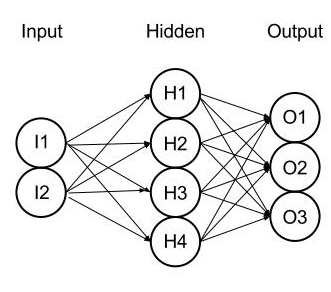
\includegraphics[scale=0.5]{mlnet.png}
	\caption{Multi-layer Perceptron}
	\label{fig:mlnet}
\end{figure}



\section{Gradient methods and backpropagation}

As with most machine learning algorithms, Neural Networks models rely on optimizations of weights $\omega$ and biases $\beta$. In order to calculate these values one should  choose a cost function that measures the variance between the actual result and the desired output on each iteration of the training phase. The two methods for running this optimization algorithm on Neural Networks are known as \textit{Backpropagation} and \textit{Gradient Descent} \cite{goodfellow2016_book}. The main goal of the algorithm is to propagate small changes $\delta$ applied to any of the neurons of the network all the way to the final layer.

\begin{figure}[h!]
	\centering
	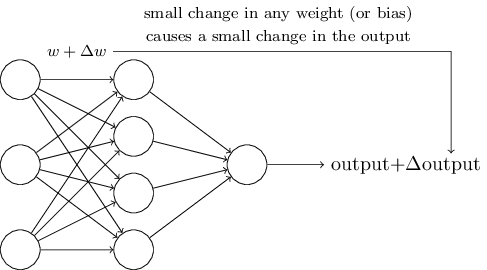
\includegraphics[scale=0.5]{net_change.png}
	\caption{Output change with regards to layer(s) weight change \cite{nielsen2016}}
	\label{fig:net_change}
\end{figure}


The network learns from data using convex optimization techniques that involves calculating derivatives of linear and polynomial cost functions. The learning algorithm should be able to find weights and biases that best approximates the output \textit{y(x)}. This approximation consists of finding the global minimum of a chosen cost function. Different machine learning algorithms require different cost functions \cite{nielsen2016}. Ultimately, one should be interested in calculating the change on the cost with respect to the weights and biases of all the neurons. This calculation makes use of partial derivatives with respect to the $\omega$ and $\beta$ in order to find the direction of the minimum for a given function $f(x)$, namely gradient \cite{goodfellow2016_book}.

$$\nabla C \equiv \frac{\partial C}{\partial \omega}, \frac{\partial C}{\partial b}$$

Gradient descent is one of the methods for finding a global/local minimum of a function. This calculation yields what is a called a gradient vector $\nabla$C which is subtracted from current weight and biases on each iteration in order to move the result towards the global or local minimum. The gradient calculation can be seen as repeatedly computing $\nabla$C, and then moving in the opposite direction "falling down" the slope of the valley.

\begin{figure}[!ht]
	\centering
	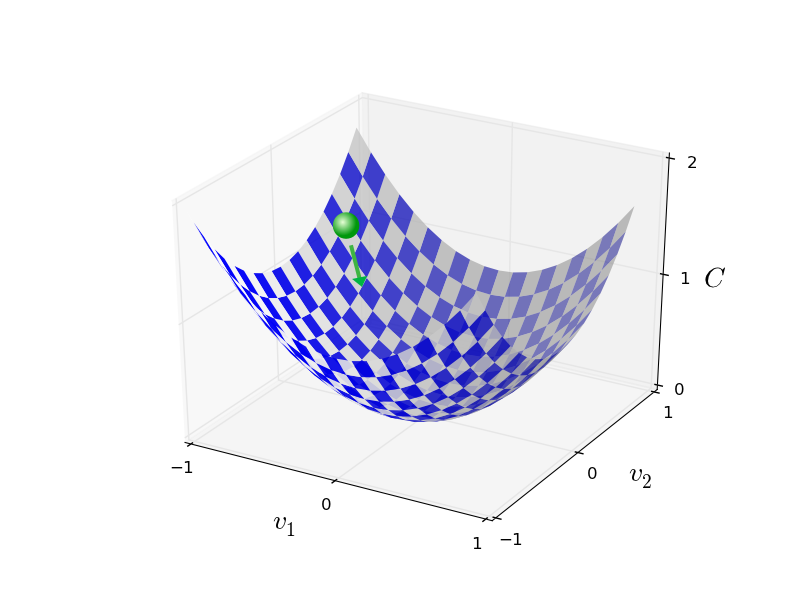
\includegraphics[scale=0.3]{valley_with_ball.png}
	\caption{Gradient calculation representation \cite{nielsen2016}}
	\label{fig:net_change}
\end{figure}

In order to learn the best representation of the input data, Neural Networks should be submitted to the optimization process where each data point is used many times to estimate the network current weights and biases. Each iteration pushes the ball into the direction of the valley by comparing a given y($x_n$) with its corresponding real $y_n$. The process should be stopped when the ball hits the lowest point of the valley, in other words, when the algorithm has converged. Mathematically speaking this is known as reaching a minimum of a function \cite{nielsen2016}. Some optimization problems are unable to find a global minimum due to their complexity, on this case, convergence is achieved by finding the local minimum.

However, when the data set is too big for running one update after a complete loop over the entire data, one should come with better strategy for updating the network parameters. Such method is that where each iteration runs on a subset of the training input namely \textit{Stochastic Gradient Descent}. One of the biggest advantages is that to speed up learning while the estimation of the gradient $\nabla$C is being computed over a subset of the data instead of all training inputs. The subset is chosen randomly on every iteration and can be referred as mini-batch. These batches are selected every \textit{epoch} and the user provides how many epochs the algorithm should run. Networks with lots of parameters can benefit the most by using a mini-batch/stochastic optimisation process.


The training of a network is performed mainly through two different types of operations: Feedforward and Backpropagation. Feedforward is the starting point of the network weights and biases optimization.The goal is to calculate the activation of each neuron from the first layer to the output layer. It involves evaluating the activation function with respect to the current weights and biases of the network by forward-propagating \textit{x} through the entire architecture. This operations yields an error $\delta$, which triggers the backpropagation part. When feedforward reaches the last layer, the error is then calculated and backpropagated to the L-1 layer. For each layer, one should find the rate of change of the cost function for each of the weights and biases with respect to its neurons. This operation is repeated subsequently until the first input layer, where the current "belief" of the network is updated making it ready for another feedforward step. The overall process should stop when there is no relevant changes in the output of the cost function.


\section{Convolutional neural networks}

Convolutional Networks are a class of deep networks that can use many layers of nonlinear or linear processing in cascade for feature extraction and transformation. They are still very similar to ordinary Neural Networks (made up of neurons that have learnable weights and biases). However, such algorithms makes the explicit assumption that the inputs are images and, therefore, are based on learning abstract representations of data with spatial properties \cite{goodfellow2016_book}. For example, an image could be represented by a vector of intensity values from 0-255 for each pixel and after being processed by the first layers of a CNN those would become more abstract representation such as set of edges, regions of particular shape and etc \cite{stanford2016}.

A convolutional neural network is different from the traditional neural network. Instead of connecting each pixel of an image, for instance, to all the neurons in the next layer, groups of pixels of fixed sizes known as patches, are connected to different groups of neurons. Each group specializes in learning specific features from the data and are not necessarily connected with all other groups in the current or next layer. The input region or group of neurons connected to a patch in the image is known as local receptive field \cite{nielsen2016}. The main advantage over shallow architectures is that the latter does not take into account the inherent spatial structure of images, in other words, all pixels are treated equally.

The main architectural difference of CNNs is that they have added some different layers to the traditional neural networks mix. The name "convolutional" originates from the convolution layer which is responsible for computing the output of neurons that are connected to local regions in the input. This operation is commonly referred in image/signal processing as a convolution between two matrices/vectors of variable sizes. The smaller regions in which the image is connected is referred as filters and/or kernels, and these would be responsible for detecting abstract features on different regions of a picture for instance. After each sequence of convolutional layers there are also the pooling layers. The main goal is to perform downsampling operation along spatial dimensions of an image (i.e width and height). This is important as an image with higher dimensions will be reduced at each layer forcing the network to learn deeper and deeper features at each iteration.

\begin{figure}[!h]
	\centering
	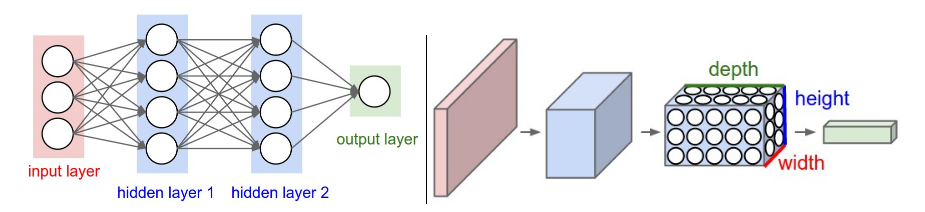
\includegraphics[scale=0.6]{conv.png}
	\caption{Shallow Neural Network vs Convolutional Neural Network}
	\cite{stanford2016}
	\label{fig:conv}
\end{figure}

CNNs are considered the state of the art solution for computer vision problems. The architecture developed by Krizhevsk et al. (2012) achieved an averaged top-1 and top-5 test set error rates of 37.5\% and 17\% where the previously record was 45.7\% and 25.7\% by a different technique. The network was comprised of eight layers, 5 of which were convolutional layers and the remaining were three fully connected layers. The output of the three last layers was fed to a 1000-way softmax to produce 1000 different image classes labels of the ImageNet dataset. Besides, max-pooling layers were also used following the fifth convolutional layer and response-normalization layers. Adding or removing any layers on this architecture yielded worst results. Overfitting was treated by using both data augmentation and dropout \cite{hinton2012improving} techniques since the architecture had over 60 million parameters. These results show that convolutional neural networks are capable of achieving above the average results even when challenging datasets with several classes are used.
\section{CNNs feature learning and visualization}

Visualizing the features of a convolutional layer helps one to understand what are the main characteristics of the input that are not only being learned but are also responsible for maximizing neurons activations cite{zeiler2014visualizing}. Until recently there was no clear understanding of why CNNs perform so well on image classification tasks. Zeiler et al (2014) \cite{zeiler2014visualizing} have produced a novel visualization technique that gives insights into the outputs of the intermediate feature layers of the network. These visualizations were then used to perform diagnostics of models and, thus, find architectures that can outperform current state of the art algorithms. One can understand that all the convolutional layers are in fact "feature extraction" layers while the fully connected ones are the actual classifier.

\begin{figure}[!h]
	\centering
	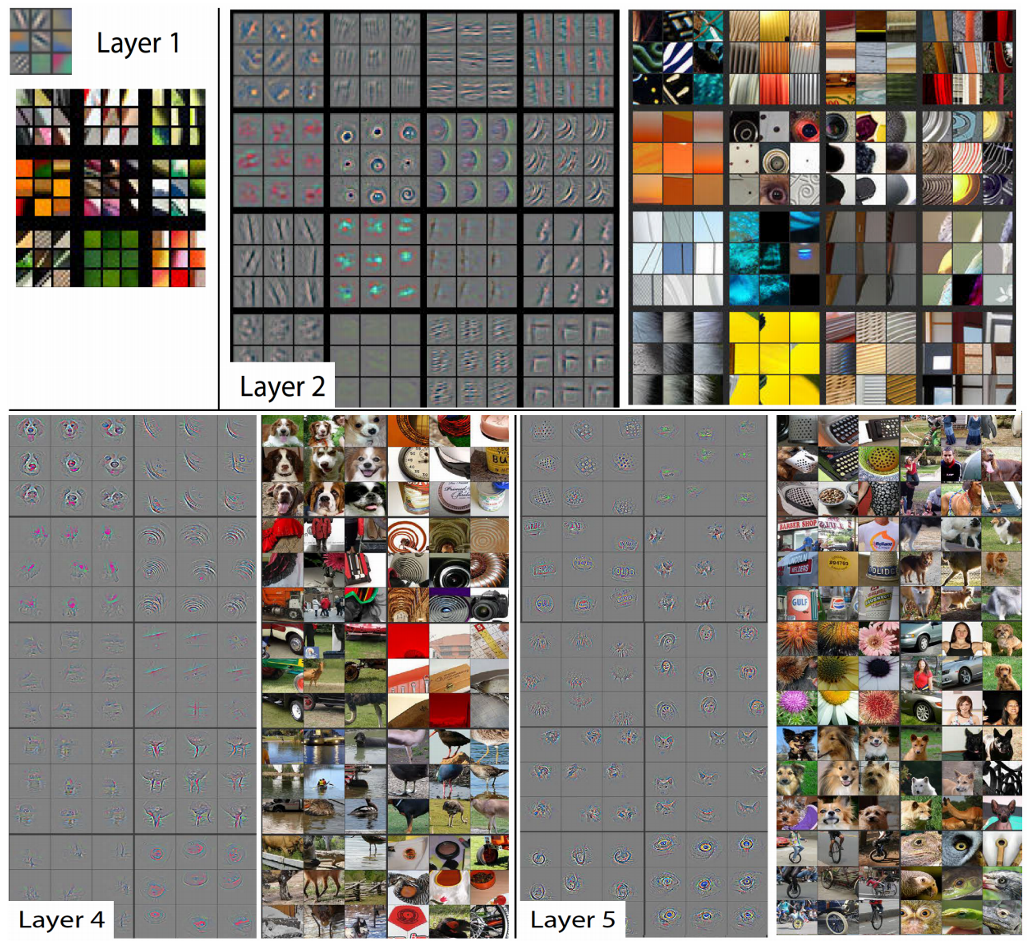
\includegraphics[scale=0.6]{layer_vis.png}
	\caption{CNN layer visualization}
	\cite{zeiler2014visualizing}
	\label{fig:conv_layer_vis}
\end{figure}

Features are learned from more abstract on initial layers to more specific and concrete on deeper layers. Figure ~\ref{fig:conv_layer_vis} shows that the first neurons are learning different types of edges while later neurons are capable of learning full representations of important regions of an image. In general these features are applicable to many datasets and tasks. As features transition from general to specific, transferability becomes negatively affected \cite{yosinski2014transferable}. For instance two similar datasets as the ImageNet and CIFAR-10 would share many common features and, therefore, a network trained on one, could be used as a pre-training or weight initialization step for another, increasing the generalization and accuracy of the model.
\section{CNNs Architectures}

The use of CNNs as a prominent technique was mainly possible due to the standardization of the dataset used for such tasks. ImageNet has become the most used classification challenge for those wanting to find better CNN architectures. The main goal of such challenges is to find models with better accuracies without focusing too much on resource utilisation. One one hand, the most important metric of a good machine learning model is its accuracy, in other words, how well it can generalize on different datasets. On the other hand, several other important metrics should be taken into consideration when using an specific CNN system in real life such as: memory footprint, parameters, operations count and etc \cite{canziani2016analysis}.

\begin{figure}[!h]
	\centering
	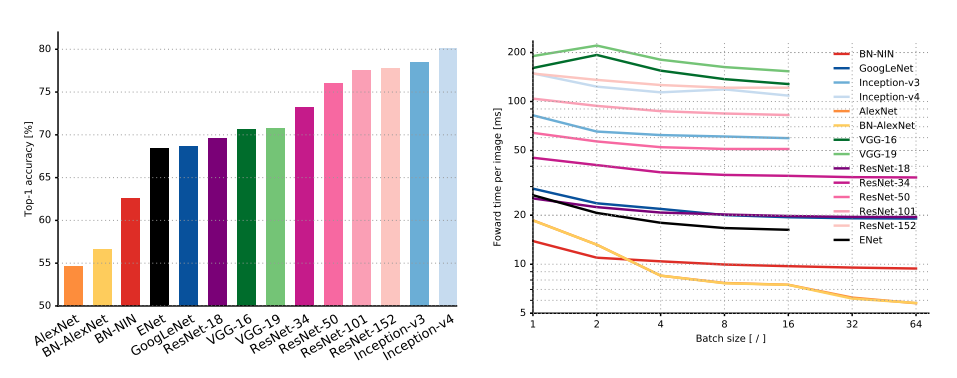
\includegraphics[scale=0.6]{network_comparison.png}
	\caption{(Left) Accuracy of Different CNN models (Right) Inference time for different batch sizes}
	\cite{canziani2016analysis}
	\label{fig:cnn_comparison}
\end{figure}

As new methods develop, one should always pick a technique that is capable of not only learning the features of the target domain but it should also fit the resource capacity of the host system. From one of the first CNN architectures (AlexNet) to the latest models (Inception V4), the accuracy has improved from $55\%$ to almost $80\%$ on the ImageNet dataset (comprised of 1.000 different class labels).

\section{CNNs properties}\label{subsec: nn_props}

Convolutional neural networks (CNNs) are considered models with high expressiveness that can achieve state of the art performance on computer vision tasks. On one hand, being highly expressive helps them to succeed but, on the other hand, it also drives them to learn solutions that are not easily understandable \cite{szegedy2013}. Usually there is a discontinuity in the input-output mappings of neural networks which can lead to miss-classification of images when the network prediction error is maximized \cite{gu2014}.The learning process of these networks through the use of backpropagation is rather complex and sometimes difficult to understand.

In order to visualize the semantic meaning of individual units, studies are currently focusing on understanding the factors leading to the activation of network neurons. It has been argued that CNNs should be stable enough to provide robustness to small perturbation of its inputs \cite{szegedy2013}. However, it has been found by mainly Goodfellow et al. (2014) and Szegedy et al. (2013) that minimal local perturbations can indeed affect the network's predictions questioning the assumption that CNNs have very good local generalization. Methods for exploiting this vulnerability were created and proven to be effective by having a very high confidence classification of adversarial examples \cite{goodfellow2016} - inputs created to deliberately yield erroneous classification outputs.

A model can achieve good generalisation by making non-local assumptions of the training inputs. Deep stacks of non-linear layers are one of the ways to have the model encoding a non-local generalisation prior over the input space \cite{gu2014}. Therefore, output units should be able to assign low probabilities to regions of the input space where no training examples are found within its vicinity. The representation of low-probability "pockets" of space on images can lead to the creation of adversaries. These are created by adding small localized perturbations on the input space which can ultimately lead to the wrong classifier outcome. 


The following chapter is going to focus on adversarial attacks and how the exploitation of the aforementioned network properties can be used to craft such examples. Three methods will be presented along with results found by different studies. Finally, methods for using this adversarial information for regularizing networks will also be shown as a possible solution for making deep neural networks less vulnerable to these kind of attacks.


\chapter{Adversarial attacks, imbalanced learning and domain shift}

This chapter focuses on how adversarial attacks are set out to successfully exploit the CNNs caveats explained in the last chapter. It starts with a study on the origin of adversaries and how imbalanced data and domain shift affect general predictive models accuracy. The discussion follows on different types of \textit{gradient sign} methods and how they use internal model information to create intentional perturbation on images. We finally end the chapter by presenting two different categories of perturbation and their interpretation on adversarial attacks.
\section{Why adversaries exist?}

Understanding why adversarial samples exists requires exploration of how learning models are built. The training data is a corpus of samples taken from an expected input distribution that are labeled according to their true class. For instance, one could have a set of e-mails classified as spam and not spam or a collection of pictures of animals where the label corresponds to each true animal type.

The integrity of CNNs is usually measured by how accurate the model is when performing a classification task. This metric is of paramount importance and, therefore, is a common target for techniques trying to exploit model vulnerabilities. Specifically, an adversary of a CNN seeks to provide an input X' that results in incorrect output classification. The degree of incorrectness in the prediction can vary and, therefore, impacts the classifier output in different ways.

Adversary types could be classified by four different categories as discussed by \cite{papernot_thesis_2016}. Confidence reduction is the adversary potential to introduce class ambiguity by reducing classification confidence. For instance, an input predicted with 99\% of confidence could have this level reduced without affecting the actual output of the model. Misclassification, on the other hand, happens when a label being previously correct is randomly changed to an incorrect output label, affecting the model output. Another different type of misclassification is to actually create perturbations using a specific target class, this method forces the model to predict towards that class. Finally, one could use the same class to create perturbations that makes the class looks less likely itself, moving the prediction outcome to the nearest class in the data space.

\section{Learning from imbalanced data}

In general, neural networks algorithms are designed to assume that the number of samples in a specific class label are roughly similar. Nevertheless, this scenario is often rare on the real world, as in most cases, the data distribution available is skewed and, hence, causes the model to be biased towards the labels with higher number of data points. This problem is known as learning from imbalanced data \cite{japkowicz2002class} and points to critical questions that are yet to be answered so one can gain deeper understanding of the vast field of machine learning. Generally speaking, there are three main approaches to learning from imbalanced data \cite{krawczyk2016learning}. 
\begin{itemize}
	\item Data-level: Aims to manipulate the data distribution by performing oversampling and undersampling operations to make it suitable for a standard learning algorithm
	\item Algorithm-level: Concentrates on modifying existing techniques to prevent bias towards majority classes and incorporate, for instance, varying penalties for each individual group of examples.
	\item Hybrid: Combines the advantages of the two previous approaches.
\end{itemize}

Even though there has been continuous development on learning from imbalanced data, there are still some new emerging challenges in, more specifically, highly dimensional data domains. As the number of dimensions of the training dataset grows, the difficulty into occupying the data space properly also increases. Varied forms of learning such as supervised, unsupervised and regression suffer from data imbalance. Moreover, extensive research on real-life applications shows that uneven data representation is an ongoing problem \cite{krawczyk2016learning}.

\section{Domain shift}



Classification accuracy should be carefully measured when training a model. For instance, the accuracy value obtained from the training set is usually higher than the one obtained from the test set. This happens when the joint distributions of training and test stages are different. A poor performance on the test set means that the divergence of both distributions (training and test domains) is high. This phenomena is usually known as domain shift or dataset shift \cite{Quionero}

Regardless of the technique, a machine learning model represents an approximation of the phenomena being modeled. In most cases the training data is unable to represent all possible input feature vectors and, therefore, can not fully capture a complete understanding of the target domain. A problem arises when the system can be exploited by providing samples that are not within the aforementioned input domain. They usually use information about the system to find where the model is inaccurate owing to missing items of the given training set.

What adversaries do is to force the domain shift in a way that the model is unable to generalize well on test data. Since data in most circumstances can not cover the entire feature space, the real decision boundary of a classification model generally becomes more complex as the phenomenon becomes more nuanced and the feature and dimension space becomes larger. This complexity is exploited by adversaries through the use of the model error as a guideline for perturbing a sample.

\begin{figure}[!h]
	\centering
	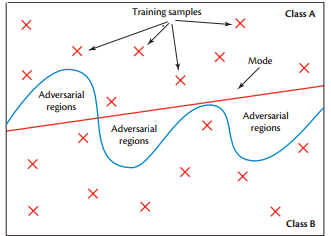
\includegraphics[scale=1.0]{adv_space.png}
	\caption{Two Dimensional Representation of unexplored adversarial regions \cite{papernot_2017}}
	\label{fig:adv_space}
\end{figure}

\section{Fast gradient sign method - FGSM}

The fast gradient sign method developed by \cite{goodfellow2014} has been used as the foundation of many of the experiments in adversarial learning on CNNs. The results have led to the conclusion that CNNs have linear behavior in very high dimensional spaces.  Most inputs were miss-classified not only on \cite{goodfellow2014} experiments but many others as well \cite{billovits, papernot2016, goodfellow2016}. This shows that adversarial examples are not hard to find. The method uses gradient information to generate image noises that changes classification outputs.
\begin{equation}
C(x + \delta)\approx C(x) + \delta * sign(\nabla C)
\end{equation}

The gradient sign equation has a simple interpretation. The main goal is to add a change $\delta$ into each pixel of the image so as to make that image closer to the chosen label on which we extracted the gradient from the source network. The sign on our $\nabla C$ indicates that we are only interested on the direction of the gradient while the $\epsilon$ controls the magnitude of the step. The method adds intentional noise that emphasizes the pixels in the image with the highest importance, so the resulting perturbation can likely lead to a misclassified result. By using the \textit(sign) function of the gradient, it is assured that the value will grow linearly with the number of the dimensions \cite{goodfellow2014}. The result of many small pixel changes is likely to generate an image with a wrong label in the network output.

The method exploits the loss function in an optimization process so one can maximize any class score for a given input image. Since everything in a CNN is differentiable it is relatively straight forward to compute the gradient information of any specific class of the input domain. The process can be done by doing a forward pass on a network with the desired class output being set to 1 in the final layer, then the backpropagation retrieves the necessary changes on gradients that would make any image looks like the desired class. 

Billovits et al (2016) summarized four different categories of adversarials generated by FGSM. True Adversarial are those given a completely different label after being perturbed. Re-Focused adversarial is the method that changes the focus of an image by giving a classification of an object that used to have lower significance while keeping the original object presence. Conaturally adversarial are those where the new output has some close relation to the miss-classified result (e.g. Dog and Cat). Finally, benign adversarial happens when the model misses the top prediction of the original image but the adversarial example gets randomly classified correctly with high confidence.

\begin{figure}[!h]
	\centering
	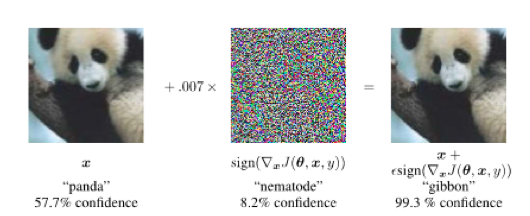
\includegraphics[scale=0.6]{panda.png}
	\caption{Adversarial example crafting with fast gradient sign \cite{goodfellow2014}.}
	\label{fig:fgsm_craft}
\end{figure}

\section{Iterative gradient sign method - IGSM}

The method from the previous section shows that small perturbations can intentionally change classifiers class labels. Sometimes, more than one iteration of the gradient sign method is required in order to have an image being incorrectly classified. By progressively applying small perturbations to an image one could achieve miss-classification of the desired sample that was not affected by one single iteration \cite{goodfellow2016}. 

\begin{figure}[!h]
	\centering
	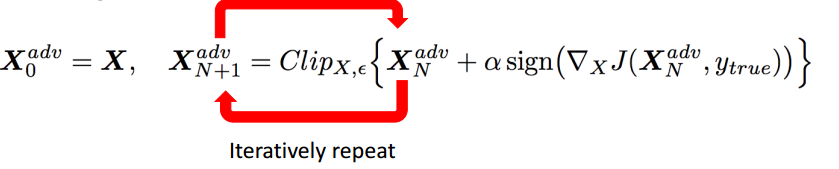
\includegraphics[scale=0.6]{iter_fgsm.png}
	\caption{Iterative FGSM Method \cite{goodfellow2016}.}
	\label{fig:iter_fgsm_craft}
\end{figure}
The extension of the fast method is reached by applying the gradient sign multiple times and clipping pixels that are not in the boundaries of the original image. Figure ~\ref{fig:iter_single_comp} shows the nature of perturbations of both methods. Since FGSM applies a single batch of perturbation to the image, it needs a higher amount of noise at a time to be able to successfully generate an adversarial.
\begin{figure}[!h]
	\centering
	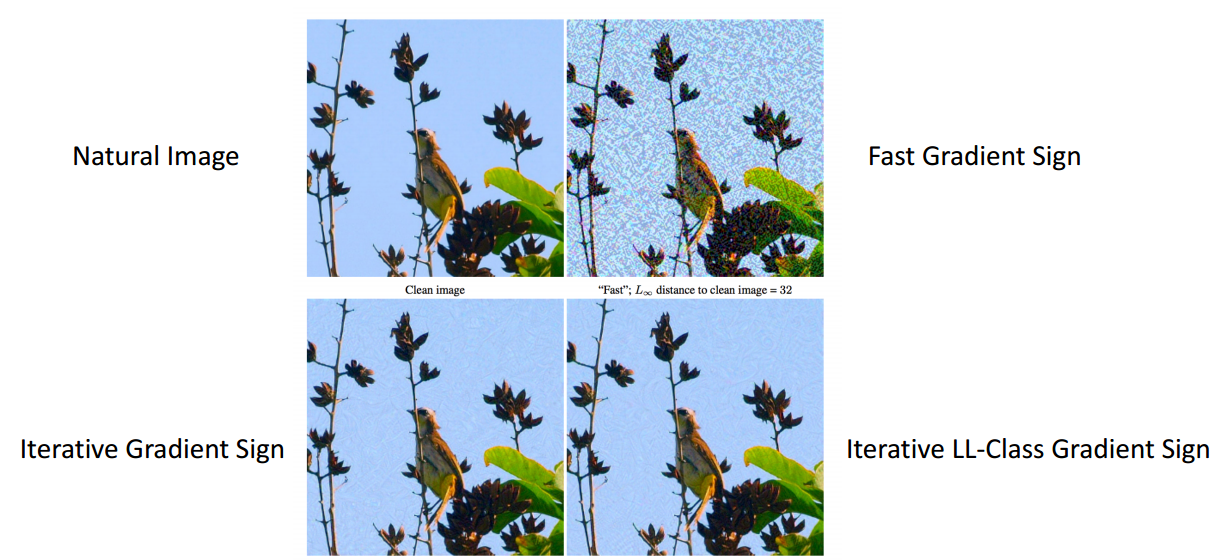
\includegraphics[scale=0.4]{iter_single.png}
	\caption{Visual Comparison of Gradients-based Methods \cite{goodfellow2016}.}
	\label{fig:iter_single_comp}
\end{figure}


\section{Ascent and descent perturbations}\label{sec:gsm}

Adding or subtracting intentional noise on images generates different adversaries,hence, requires different interpretations. By adding noise to an image, one would be making the gradient to go "uphill" and therefore moving away from the desired class, this results in an increase in value of the loss function and thus should be referred as the \textit{ascent method}. On the other hand, when subtracting intentional noise, one would be doing a process similar to the optimization of a loss function where we approach the minimum of a function and, thus, we get closer to the desired class, this approach is hereby known as the \textit{descent method}. These approaches can be coupled with iterative methods or fast methods to take progressive/single steps towards or away class labels. Some images/classes can be more robust to these perturbations and would, therefore, require more iterations or more noise from the gradient methods. Equations ~\ref{eq:ascent} and ~\ref{eq:descent} shows both ascent and descent methods 

\begin{equation}\label{eq:ascent}
C(x + \delta)\approx C(x) + \epsilon * sign(\nabla C)
\end{equation}
\begin{equation}\label{eq:descent}
C(x + \delta)\approx C(x) - \epsilon * sign(\nabla C)
\end{equation}
\chapter{Attacking machine learning systems}

In this chapter, we present approaches for attacking machine learning algorithms with adversarial techniques presented in the previous chapter. We discuss that the knowledge of the architecture and weight parameters is sufficient to derive adversarial samples against CNNs. Further discussion goes into black box attacks where the attack has minimal information about the underlying system. The chapter is then concluded with how model's knowledge can be transferred between different algorithms/techniques.


\section{Transferability}

Papernot et al. (2015) has shown that many adversaries created to fool one specific model are also likely to affect another different model. As long as the models were trained to perform the same task, knowledge can be transferred when querying the victim model, namely oracle, to label a synthetic training set for the substitute.

The transfer learning phenomena constitutes a threat vector for many state of the art methods, thus, one should be able to quantify most vulnerable classes of models by generating accurate comparison of the vulnerabilities of each class. Attacks can, however, depend on some specific information of the target as shown in Table ~\ref{tbl:attack_info}. Techniques can mainly be split into both Intra-Technique and Cross-Technique. These are discussed in more details on the following sections.

\vskip 1cm

\begin {table}
\begin{tabular}{|c|c|}
	\hline 
	Model Parameters (Weights and Biases) & Have full access to model wieghts \\ 
	\hline 
	Model Architecture / Type & Know what the model looks like \\ 
	\hline 
	Training data & Understand the data domain \\ 
	\hline 
	Oracle/Black box & Query model with input X, get label Y \\ 
	\hline 
	
\end{tabular} 
\caption {How Much Information is needed to fool a model?}
\label{tbl:attack_info}
\end {table}

\medskip



\section{Intra-technique transferability}\label{sec:intra}

The Intra-technique transferability is achieved by reproducing the learning process between two identical algorithms \cite{papernot2016transf}. Even though, the algorithms can differ in terms of architecture, they are still based on the same fundamental learning concept. For example, most learning algorithms could be categorized into three general classes: differentiable algorithms like CNNs and Logistic regressions, lazy learners like KNN and non-differentiable models like SVM and Decision Trees. Therefore, this technique consists of keeping the same learning method while differing the hyperparameters/architecture and using queried subset of the training data to train the local model. 



In order to make a comparison between these techniques, \cite{papernot2016transf} created five different dataset models of the MNIST to train the algorithms and compare how they performed when using different and same models of training data. All models had non-negligible vulnerability to this kind of approach. While the CNN and the logistic regression were highly vulnerable to these attacks, SVM, DT and KNN were more robust achieving better overall resilience. The results have led to the hypothesis that non-differentiable techniques are more robust to black-box attacks using locally generated adversarial sample with two algorithms of the same type \cite{papernot2016}. Figure ~\ref{fig:intra} shows classification performance when using intra-technique methods.

\begin{figure}[!h]
	\centering
	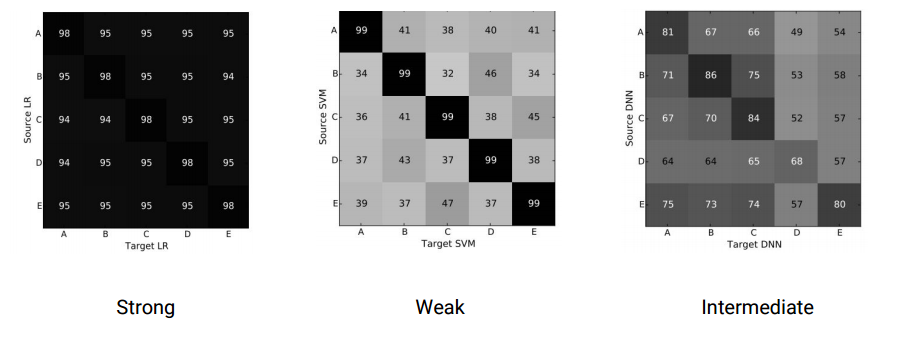
\includegraphics[scale=0.6]{intra.png}
	\caption{Knowledge transfer level using Intra-Technique Transferability \cite{papernot2016transf}}
	\label{fig:intra}
\end{figure}


\section{Cross-technique transferability}
Cross-technique transferability is referred as the knowledge transfer between two different machine learning techniques. This technique has a higher degree of difficulty than the method shown on section \ref{sec:intra} as it involves models using possibly very different techniques like DNNs and Decision trees. Yet, this can be seen as quite strong phenomenon to which techniques like Logistic Regression, Support Vector Machines and Decision Trees along with Ensemble based models are extremely vulnerable \cite{papernot2016transf}. While DNN's ended up as being the most robust of the methods with misclassification rates varying between 0.82\% and 38.27\%, Decision Trees were the most vulnerable with rates from 47.20\% to 89.29\%. Interesting enough, ensemble methods -- focused on measuring the output of all the "experts" in the group -- have shown quite vulnerable to the experiment. The hypothesis is that the technique explores the individual vulnerability within each of the ensemble methods.

\begin{figure}[!h]
	\centering
	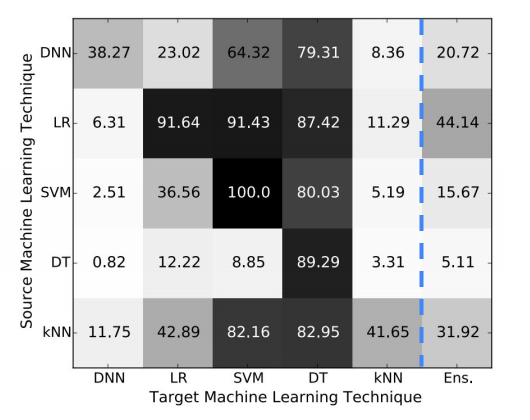
\includegraphics[scale=0.6]{cross.png}
	\caption{Knowledge transfer using Cross-technique transferability and Ensemble methods \cite{papernot2016transf}}
	\label{fig:cross}
\end{figure}
\section{Black-box attacks}
Black-Box attacks to machine learning systems alleviates the dependence on knowing both victims training data and model information. This method solely depends on accessing the label assigned by the target for any chosen input. The strategy consists of learning a substitute for the target model using a synthetic dataset generated by the adversary and labeled by the observed victim, namely here, the Oracle \cite{papernot2016}.

Training the substitute model that approximates the Oracle poses some challenges. Selecting an architecture for the substitute ends up in being an arbitrary process, as one should try different models and evaluate the one with the best result. Generating the synthetic dataset needs to limit the number of queries sent to the oracle so the approach is tractable. 

Experiments from Papernot et al. (2016) were performed against real-world remote systems in order to validate the effectiveness of such attacks. The results have shown that systems using DNNs are usually more robust and require more queries to have the substitute being able to generate samples that are misclassified by the oracle.

\begin{table}[!h]
	\centering
	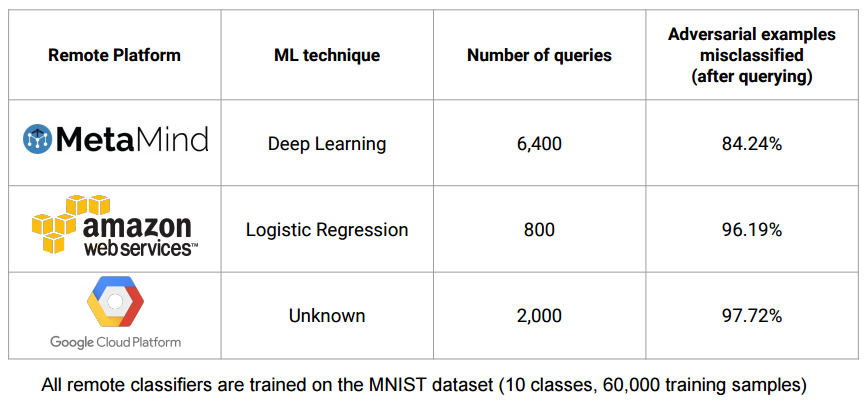
\includegraphics[scale=0.7]{black_box.png}
	\caption{Black-Box attacks results against real world systems}
	\label{tbl:black_box}
\end{table}

\section{Unrecognizable images}\label{subsec:unrec}

Adversaries, on the other hand, are not restricted to small perturbations on known images. The work of \cite{nguyen2015} presented a method for producing images that are unrecognizable to humans, but are nonetheless labeled as recognizable objects by DNNs. For instance, a DNN would classify a noise-filled image crafted using their technique with high confidence. These images not have a source class but are crafted solely to perform a targeted misclassification attack.

\begin{figure}[!h]
	\centering
	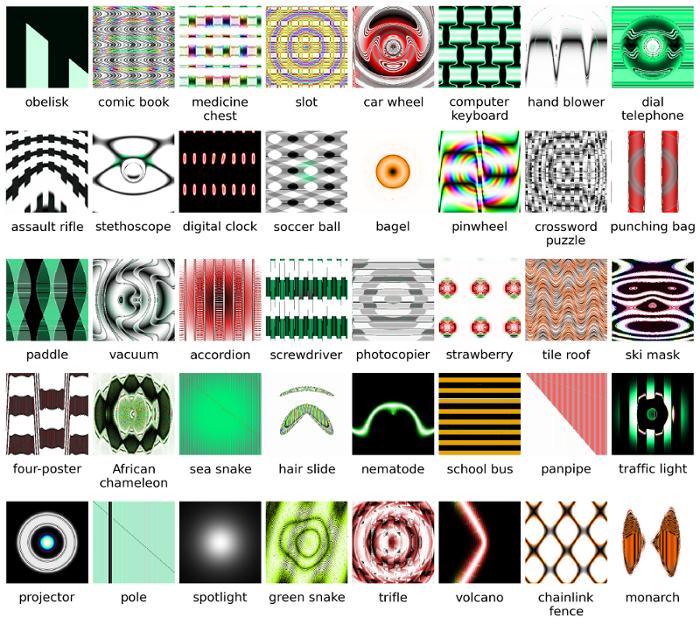
\includegraphics[scale=1.]{unrec_images.png}
	\caption{Examples of noisy images classified with high confidence \cite{nguyen2015}.}
	\label{fig:unrec_images}
\end{figure}


\section{Adversaries in the physical world}\label{sec:physical}

All the aforementioned techniques rely on feeding information directly into the targeted machine learning systems. Such models only takes into consideration situations in which attacks take place entirely within the computer. For instance, these techniques could be used by attackers to avoid spam filters or malware detectors. Even though the study of adversaries in the digital world is utterly relevant, a recent study conducted by \cite{goodfellow2016} have shown that it is possible to craft adversarial samples so as to perform attacks on machine learning systems which are operating in the physical world.

Although the \textit{gradient sign} method have been successful on crafting adversarial examples, there are some extensions of the method that can be used in order to create perturbations that are more likely to work in the physical world. Goodfellow et al. (2016) introduced a variation of the perturbation method named \textit{Basic Iterative Method}. This technique applies the fast gradient method multiple times with small step sizes and makes sure that all pixels are within a $\epsilon$-neighbourhood of the original image. The number of iterations was chosen heuristically with goals of being sufficient enough to have the adversarial example reaching the edge of the $\epsilon$ max-norm.

In order to create a physical world setting in the experiment, clean photos of adversaries were created using different gradient sign methods and then fed into a machine learning system using a CNN (Inception V3). Adversarial Images created using the fast method were more robust when compared to the iterative methods. The explanation of the result is that iterative methods create more subtle perturbations that can be easily be destroyed by the photo transformation process. Overall, it could be expected that about 2/3 of the images would be top-1 misclassified and about 1/3 top-5 misclassified by the fast method using an $\epsilon$ of 16.

Adversarial examples is not only feasible on digital attacks but also on physical world scenarios. By using the correct perturbation algorithm with optimized hyperparameters one can use printed digital photos to fool day-to-day machine learning systems. As more and more machine learning is becoming part of our environment, techniques for avoiding such attacks need to be developed so these systems can become less vulnerable to any kind of attack.

\section{Defending against adversarial attacks}\label{sec:robustness}

Since adversarials are exploiting intrinsic network properties, these fake inputs could also be used when training a network in order to develop robustness to examples created using the same methods. By using the worst case perturbation of a point \textit{x} instead of \textit{x} itself it is shown on equation ~\ref{eq:adv_train} that the perturbation is included within the model's objective function. This form of training was able to reduce the error rate of adversarial examples from 0.94\% to 0.84\% \cite{goodfellow2014}. Adversarial training can be seen as a way of teaching the model how an adversarial looks like and that it should be able to generalize not only normal images but also perturbed ones. Another approach was developed and it uses Bayesian non-parametric methods. Estimating the confidence that an input is natural during the training phase can lead the network to generate priors that take into account adversarial perturbation of points \cite{billovits}. 
\begin{equation} \label{eq:adv_train}
C(\omega,x,y) = \alpha C(\omega ,x,y) + (1-\alpha )C(\omega ,x+\epsilon sign(\nabla_{x}C(\omega,x,y))
\end{equation}

Most adversarial crafting techniques use the gradient of the model to make an attack. In other words, they look at a picture of an airplane, they test which direction in the feature space makes the probability of the "cat" class increase, and then they give a little push in that direction. These are hard to defend against because it is hard to construct a theoretical model of the crafting process. These examples are solutions to an optimization problem that is non-linear and non-convex for many ML models, including neural networks. Since there is no good theoretical tool for explaining the solutions of these complicated problems, it is very hard to make any kind of theoretical argument that a defense can improve an algorithm from a set of adversarial examples.
\chapter{Experiment design} \label{chap:experiment}

This chapter presents the experimental environment used during the development of this work. The first two sections will focus on discussions around the choices of data domain and the CNN architecture. The next section explains all the networks variants, techniques and parameters chosen for training. The two subsequent sections are dedicated to explain the reasons behind the perturbation method and the synthetic generation of the imbalanced dataset, which are the core ideas behind this work.
\section{Data domain}

Our experiments aims to investigate the relationships of the underlying learning structure of CNNs and the perturbation caused by gradient sign methods. In particular we focus on the investigation of how the gradient step from the sign method moves the points away from their distributions, and how this could be affected by both balanced and imbalanced training sets. This requires  class labels of the data set to be non-hierarchical so we can make better assumptions of their distributions. 

We use the CIFAR-10 data set \cite{krizhevsky_2009} in our experiment. CIFAR-10 data is visually rich and empowers the analysis between different class labels. The data set contains 32x32 images in 10 classes, each has 5,000 samples for training and 1,000 for testing. There is not much overlap nor hierarchical relationship between classes. Most CNNs experiments nowadays uses the 2014 ImageNet dataset \cite{deng2009imagenet}. However, its hierarchically organized categories adds unnecessary complexity to the experiment design hindering the analysis of the results (e.g. causality relationships).
\section{The VGG architecture}

As described in Chapter 2, a CNN is a sequence of layers where every layer transforms one volume of activations to another through a differentiable function. Three main types of layers are used to build these networks: Convolutional Layer, Pooling Layer and Fully-Connected Layer. A Convolutional Layer computes the output of neurons that are connected to local regions in the input, the Pooling layer performs down-sampling operations along the spatial dimensions of the input and, finally, the Fully-connected layer computes the class scores of the classifier. The chosen architecture should have enough layers for learning good features from the training set domain. For instance, a CNN Architecture for CIFAR-10 could have the following configuration: [INPUT - CONV - RELU - POOL - FC].

Network architectures with higher accuracies are able to diminish the effects of domain shift, however, adversaries are efficient into extrapolating the given domain by going to previously unseen regions of space. For this work we have chosen a network architecture that not only provides reasonable accuracy for our selected dataset (CIFAR-10) but it is also reasonable on resource consumption. On this way we can reproduce the requirements of a real world system where not only accuracy is taken into account when selecting a CNN model.

From all CNN architectures tested on Canziani et al (2016), the VGG16-19 from Simonyan et al. (2014)  seemed to have the best trade off between accuracy and performance (inference time). The VGG architecture won the first and second places on the ILSVRC-2014 submission on the localisation and classification task. The main contribution of the VGG network was to show that the depth of the network is a critical component for good classification performance. The model can be assembled with 16 or 19 Conv/FC layers and it features an extremely homogeneous architecture that only performs 3x3 convolutions and 2x2 pooling from beginning to end.

\begin{figure}[!h]
	\centering
	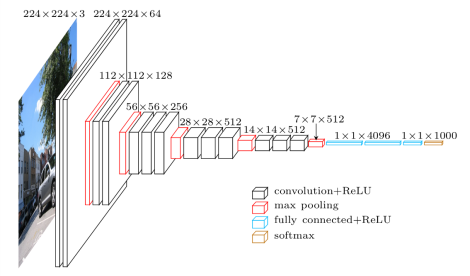
\includegraphics[scale=0.6]{imagenet_vgg16.png}
	\caption{VGG16 on ImageNet}
	\cite{simonyan2014very}
	\label{fig:vgg16}
\end{figure}

The design of the VGG16 has been proven to work even on datasets with several classes that are very different from each other . The two last fully connected layers of the state of the art model are comprised of 4096 neurons each, leading to much higher parameters complexity. As the dataset used in this work has only 10 classes, the two FC-4096 layers were replaced by one single layer with 512 neurons and RELU activations. This helped to reduce over-fitting when training the network. In addition, the total number of convolutions blocks and pooling were reduced to 3, with the first layer having 2 stacked convolution layers followed by a max pooling of stride 2x2 and the last two layers with 3 stacked convolutions also followed by a max pooling of stride 2x2. The max pooling layers are responsible for reducing the image size by 50\% every time an image passes through it. Since CIFAR-10 images are only 32x32, the original VGG16 architecture would end up having an output of shape of only 1x1 pixel at the last layer. In order to avoid this problem, the number of layers were reduced so as to fit our dataset specifications. The resulting shape fed into the fully connected layers is 4x4x128 (Width x Height x Channels) as it can be seen on table ~\ref{tbl:vgg10}. 

\begin{table}[!h]
	\centering
	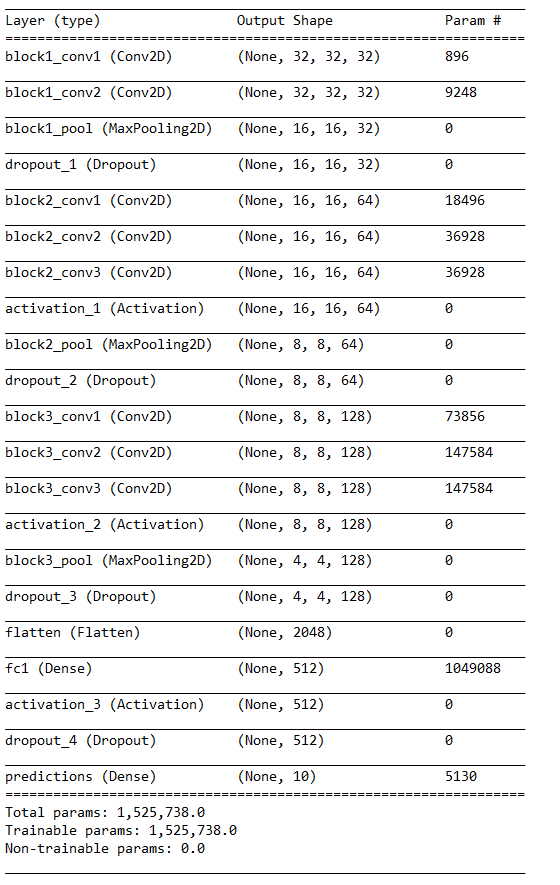
\includegraphics[scale=0.9]{vgg_arch.png}
	\caption{Full Model Description}
	\label{tbl:vgg10}
\end{table}

\section{Overall training process}

Convolutional neural networks (CNNs) require good optimisation methods in order to unleash their full potential. As networks get deeper, the number of resources required to train increases considerably. CNNs can share parameters within its convolution layers, thus, reducing the amount of computation needed during the training stage. All the models in this work were implemented using Python programming language along with Tensorflow and Keras frameworks. The first is a high performance calculation engine that uses GPUs to accelerate its matrix/vector calculations. The latter is a Neural Network library that helps on the implementation of any deep learning model. Keras is mainly a wrapper on top of Tensorflow that hides algorithms complexity from the developer, making it one of the best frameworks for CNNs currently.

As discussed on Chapter 2, the full gradient update would not be the best choice for optimizing deep networks. Stochastic Gradient methods were one of the first methods developed to overcome this problem and are still being further developed nowadays. The SGD based optimisation technique used in this work was developed by Bengio (2015) \cite{bengiormsprop}, namely RMSProp. This method is an adaptive learning rate scheme that can take the absolute values of the Hessian's eigenvalues and, therefore, approximate the equilibration pre-conditioner. As shown on Bengio's work \cite{bengiormsprop}, the method outperforms current SGD methods by achieving convergence faster. The learning rate for the method was set at $10^{-4}$ and the decay $10^{-5}$.

In order to achieve optimal accuracy, every algorithm should be trained until convergence, in other words, it does not under-fit or over-fit the given dataset. Avoiding over-fitting and under-fitting is highly important when training CNNs. Our architecture was trained until no more reasonable changes were detected in the validation loss so we could dismiss unnecessary training steps and consequently any kind of over-fitting. This was achieved by using the Early Stopping technique as described on \cite{stanford2016}. Fundamentally, this consists of a functional callback that runs at the end of every epoch and compares the previous loss with the current one and interrupts training if the difference was below an user provided $\delta$ for a specific number of steps in a row. The value of our $\delta$ was set at $10^{-4}$ and the number of steps to 10. For instance, training would be stopped if no improvement over the specified $\delta$ was seen for 10 steps in a row.

\begin{figure}[!h]
	\centering
	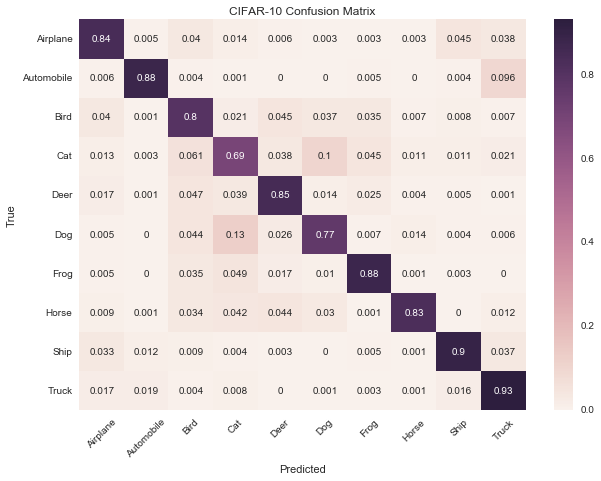
\includegraphics[scale=0.6]{conf_matrix.png}
	\caption{Results on the full dataset}
	\label{fig:conf_matrix_full}
\end{figure}

The confusion matrix helps understanding the individual score for each class and also provides information of the ratio on which the true class was misclassified as other classes. Figure ~\ref{fig:conf_matrix_full} shows that the Cat and Dog classes are often interchangeably misclassified as they have a set of similar features. The network have reached an overall accuracy of 83.45\% and a total validation loss of 0.5033.

\section{Perturbation method}
The gradient sign is a method that uses internal gradient information to create directed perturbation to input data. The resulting label will be different whether one adds or subtracts noise according to equations 1 and 2. 

\begin{equation}
C(x + \delta)\approx C(x) + \epsilon * sign(\nabla C)
\end{equation}
\begin{equation}
C(x + \delta)\approx C(x) - \epsilon * sign(\nabla C)
\end{equation}
Suppose the current true label of the class is selected as a gradient candidate, adding noise would mean that we increase the cost function of our input while subtracting noise is the same as minimizing our loss function even further. The equations above are usually referred as ascent and descent methods
\begin{figure}
	\centering
	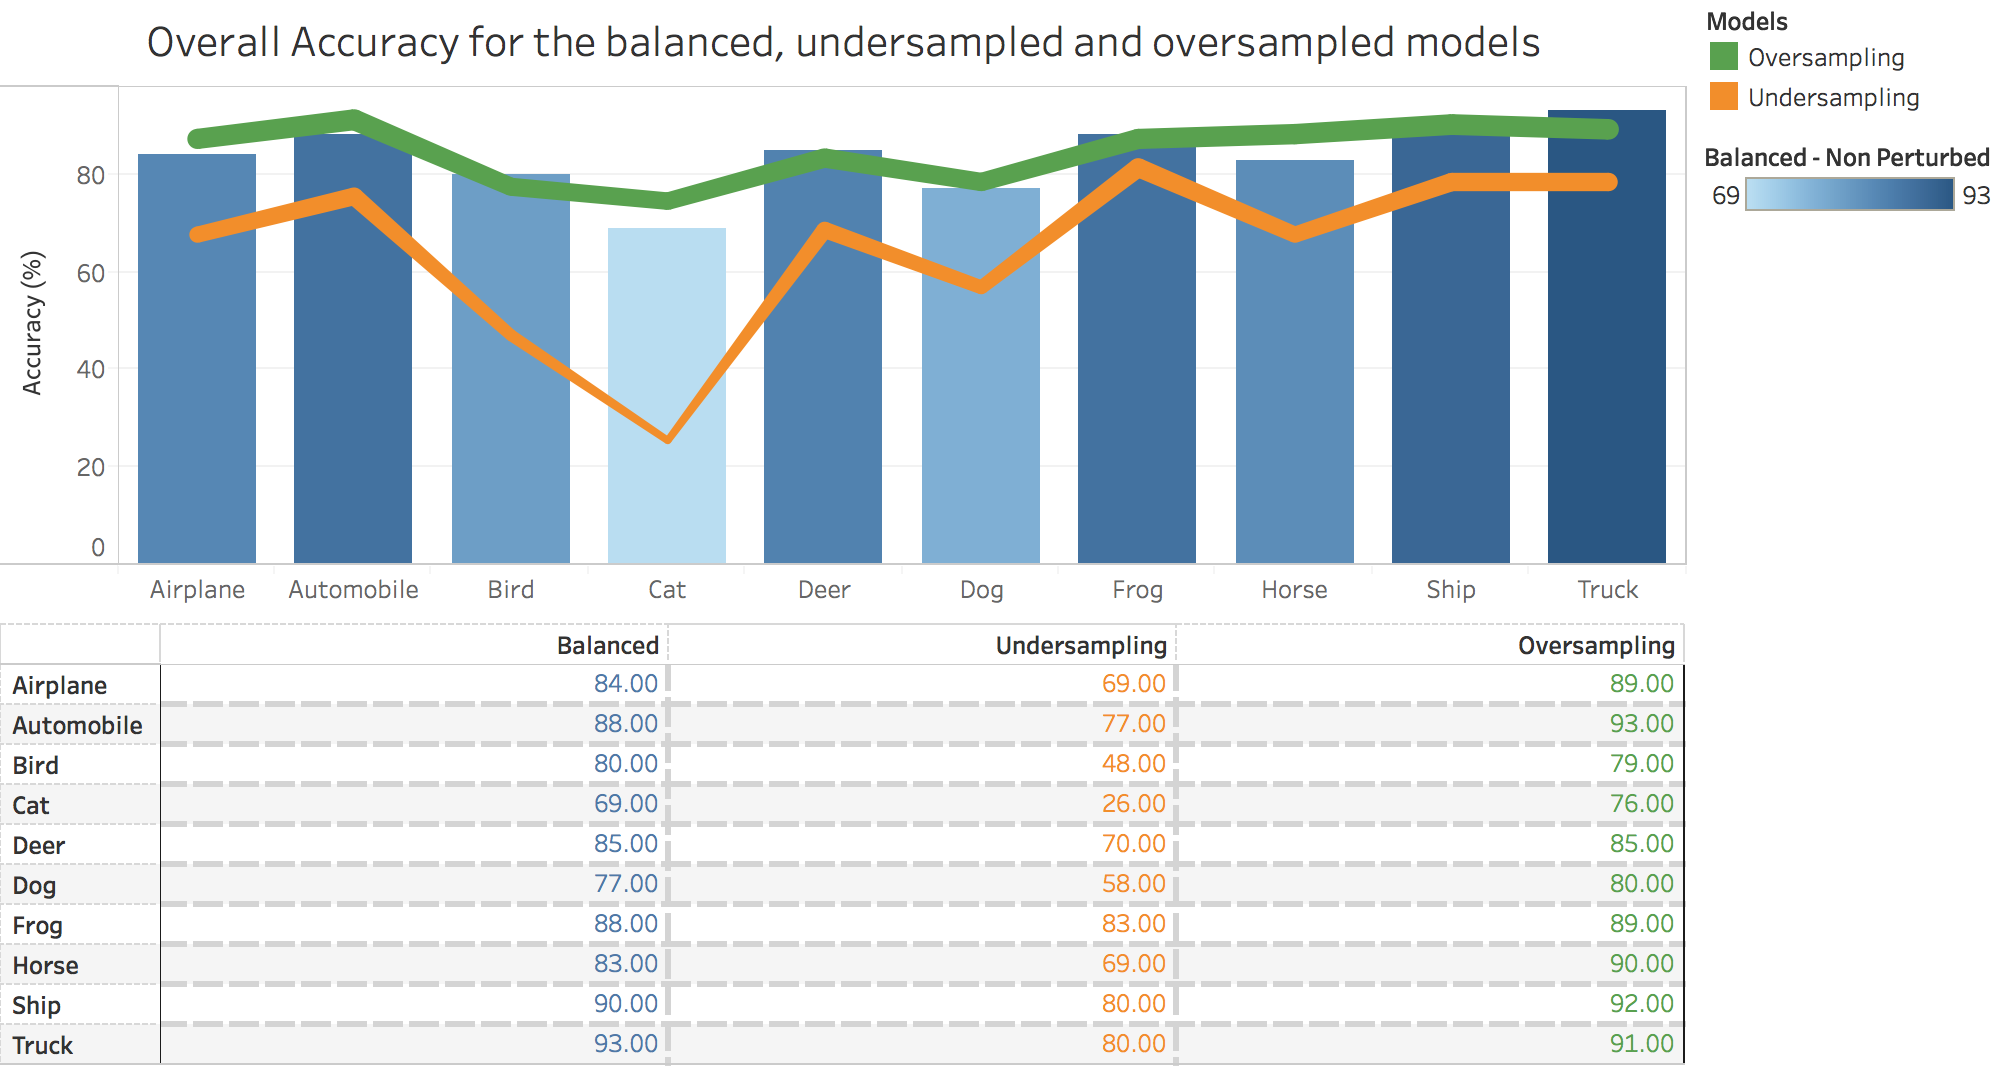
\includegraphics[height=6.5cm]{graph_non_pert.png}
	\caption{Individual class accuracy for under-sampled, over-sampled case on the CIFAR-10 modified dataset shows a decrease in accuracy for classes with lower number of samples}
	\label{fig:acc_graph}
\end{figure}
In order to enforce consistency throughout our experiments, we have chosen the true sample label as the backpropagated gradient along with the fast gradient sign ascent method. The intuition behind this choice is that we look to increase the cost function of the target class by moving away from the current true label. The $\epsilon$ value chosen was 0.01 as it provided the best trade=off between misclassification and the amount of visible change applied to the input image.

\section{Synthetic data imbalance}

Classification models are usually required to have similar number of samples for each class in order to equally learn proper feature representations for each label. As shown on Murphey and Guo (2004) \cite{murphey2004}, Neural Networks have lower generalization capabilities and are biased towards specific classes when trained on datasets with unequal number of samples between classes. 

As the CIFAR-10 dataset is not naturally imbalanced, we have artificially created two variations on which we trained the imbalanced networks.  One dataset consists of a direct under-sample of the target class to 1,000 samples, and the other was created using  an over-sampling of the target class (or an under-sampling of all other classes). We kept the number of samples for the target class at 5,000 while all other classes were reduced to 1,000 samples. For each class of the two different datasets configurations, a network was then trained until convergence using the same hyper-parameters as the balanced case. Each model was evaluated against a test set of 1,000 samples of the target class which was perturbed by its own under/over-sampled model and the balanced model. The two sources of gradient information are referred as white-box and black-box attacks since the former has complete information of the network weights and biases while the latter uses an approximation of the same parameters. 

Both imbalanced networks were separately tested for each class on white-box and black-box adversarial attacks. The white-box test was designed to investigate the vulnerability of class imbalance on adversarial examples while the black-box test is designed to verify the robustness on transfer learning environments. In total we evaluated 50 different combinations: 20 for each different imbalanced dataset (same model gradient and balanced network gradient) and 10 for the balanced network using its own gradients on each class. Figure~\ref{fig:acc_graph} shows the accuracy for the models without any perturbation. It can be seen that the individual class accuracy for the under-sampled case is reduce while the same metric is increased on the over-sampling network. 

\begin{figure}[!h]
	\centering
	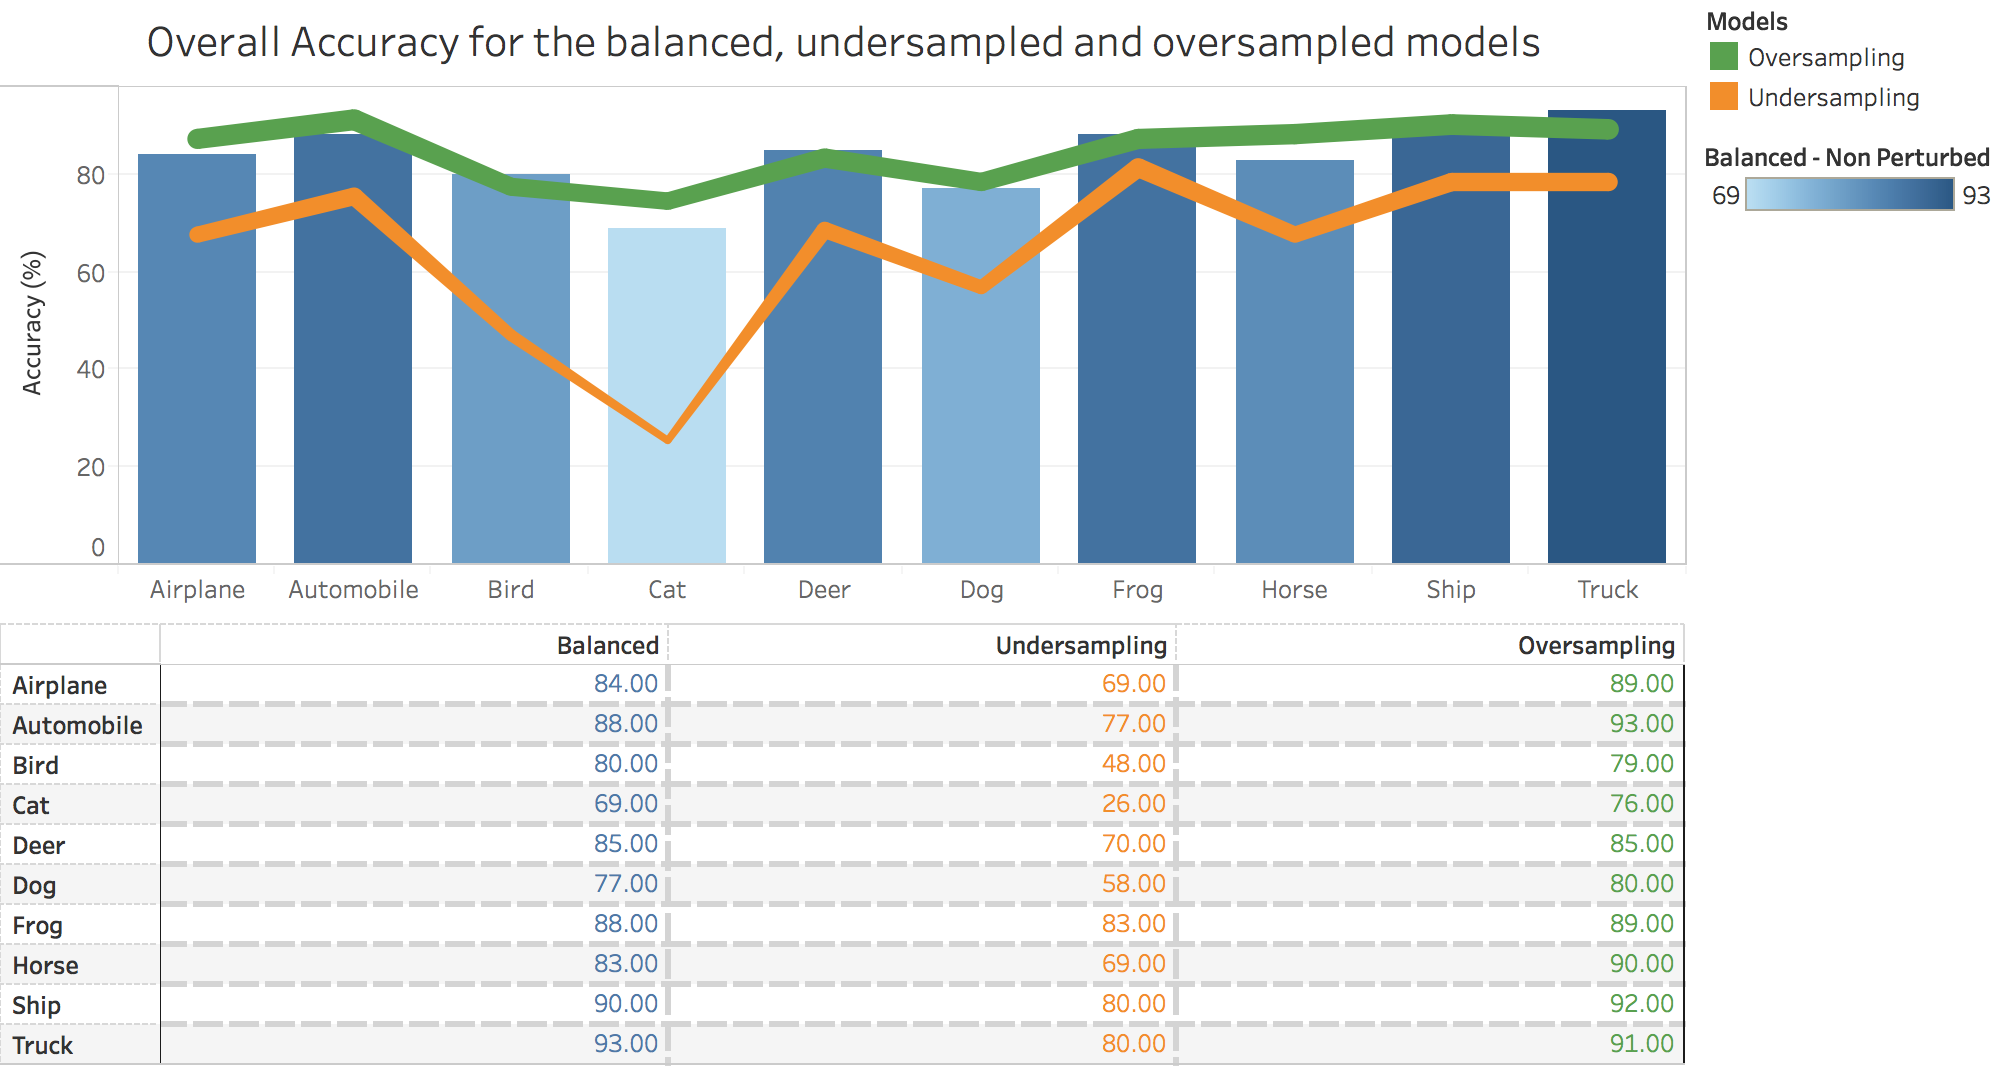
\includegraphics[scale=0.3]{graph_non_pert.png}
	\caption{Target class accuracy on all models}
	\label{fig:acc_graph}
\end{figure}

Figure ~\ref{fig:acc_graph} shows the per class accuracy for each specific model on non-perturbed test set. While the over-sampling on the target class causes the per class accuracy to increase, the down-sampling causes the same accuracy to be drastically reduced when compared to the balanced model shown on figure ~\ref{fig:conf_matrix_full}. The former happens because the model learns more about the target class due to its increased number samples, hence, it concentrates on learning the specifics of the class rather than equally splitting its capacity through all classes as it happens on the latter. The increased accuracy means that the model better explores the space around the target class since it does not have enough evidence to explore other classes feature spaces.


\chapter{Results} \label{chap:results}
In this chapter we present the results from our experiments on different types of imbalanced datasets. We first start by showing the results on the balanced model so as to set the baseline of comparisons. A discussion then follows on the under-sampled and over-sampled cases and transfer learning results for perturbations with different models. The chapter is then concluded with the results for the cases where classes have similar features, and, therefore, share overlapping distributions.

\section{Baseline model}
Canonical models assume that every object in the dataset are sampled from similar distributions. However, in real-life situations, even though the number of samples is the same for each label, they could still be poorly represented by the lack of a clear structure. This often leads to differences in the output for each specific class \cite{krawczyk2016learning}. On this way, a superficially balanced dataset does not guarantee that the model will equally generalise across all classes.We use the results of the balanced network on adversarial attacks as the baseline
to evaluate whether imbalanced CNNs are more or less vulnerable to these malicious methods.

Table ~\ref{tbl:results} shows that the accuracy for all classes is drastically reduced when the balanced model is presented with adversarial inputs. Even though there is equally distributed number of samples for each class, the adversarial attack forces the domain shift of each individual sample towards different regions in space, causing a misclassification of the current label. Cat and dog classes are conatural adversaries according to \cite{papernot2016} and they presented the lowest accuracy of all classes with 11\% and 15\% respectively. As both labels have distributions that overlap, the sign method becomes more effective since the distance between them is smaller. 
\begin{table}
	\centering
	
	\begin{tabular}{lccccc}
		\toprule
		&\multicolumn{2}{c}{Different Model}
		&\multicolumn{3}{c}{Same Model}
		\\\cmidrule(r){2-3}\cmidrule(l){4-6}
		Class Label &Undersample &Oversample &Balanced &Undersample &Oversample \\
		\midrule
		0 - Airplane &60\%& 87\% &36\%& 19\%    & 61\% \\
		1 - Automobile &64\%& 91\% &23\%& 16\%    & 63\% \\
		2 - Bird &38\%& 73\% &20\%& 9.4\%    & 27\% \\
		3 - Cat &21\%& 72\% &11\%& 0.5\%    & 19\% \\
		4 - Deer &58\%& 80\% &20\%& 9.8\%    & 20\% \\
		5 - Dog &47\%& 76\% &15\%& 9\%    & 38\% \\
		6 - Frog &76\%& 88\% &27\%& 20\%    & 49\% \\
		7 - Horse &59\%& 88\% &20\%& 18\%    & 52\% \\
		8 - Ship &69\%& 89\% &37\%& 19\%    & 59\% \\
		9 - Truck &46\%& 87\% &49\%& 21\%    & 54\% \\
		\bottomrule
	\end{tabular}
	\caption{Results for the two different sources of perturbations along with the two different imbalanced datasets}
	\label{tbl:results}
\end{table}
\section{Under-sampling and over-sampling models}

The results on both under-sampled and over-sampled models has shown some interesting properties of adversarial attacks. 
Table ~\ref{tbl:results} illustrates that models with under-sampled datasets were more vulnerable than balanced models. Figure ~\ref{fig:relative_difference} shows the relative difference for all the three different networks (balanced, under-sampled and over-sampled). Values were calculated by finding the difference between the perturbed accuracy and the non-perturbed accuracy of each class model. They represent the percentage on which the initial accuracy was reduced. The under-sampled model had the higher relative difference on average, which shows that the imbalanced nature of the dataset ended-up increasing the vulnerability to adversarial attacks.

Even though the vast majority of results has shown higher vulnerability of the under-sampled models, some results are worth to discuss. For instance, the deer class has shown the same relative difference on both over-sampling and balanced model cases, which indicates that more samples are not necessarily adding more information to the class distribution. Further causality relationship could be established by looking at individual samples of the class to investigate if they are similar to one another so as to justify this result. However, if thats not the case, another hypothesis is that individual samples provide high quality information about the class and thus makes the model learning process on that class more effective. The dog and frog cases presented similar patterns between all three models while the cat class was the highest relative difference of all classes. 

Perturbation on the over-sampling case, has shown less effective on the majority of classes. The small push caused by our $\epsilon$ was not enough to move points to outside of their distributions. Objects of the over-sampled classes would need bigger steps in order to successfully create an adversary that leads to a wrong classification label. Accuracy for
most of the over-sampling cases was around 45\% and the relative difference was the lowest of all three models, which shows robustness of the target over-sampled class.For instance, airplane and automobile perturbations have reduced the initial accuracy by only 31.46\% and 32.26\$ respectively, which shows that over-sampling on these classes has helped to model to establish better decision boundaries during optimisation.

In order to better understand these results, we need to study how decision boundaries of models are established. Class imbalanced models are naturally affected by the false positive and false negative trade off shown on figure \ref{fig:class_dist}. The decision boundaries on such models favour the class with more samples and, hence, increases the accuracy for one class while decreasing for the other class. The area under the curve for misclassified examples on the under-sampled distribution is bigger, and it is caused by the suboptimal exploration of feature space of that class. This effect is exploited by adversaries as there is an increase on the misclassification rate of distributions with lower amplitude. An under-sample of a specific label causes its distribution to be squished into space and, hence, have less impact on the definition of decision boundaries.


The increased number of samples of the over-sampled label, causes the network to perform the aforementioned trade-off when optimizing its loss function. For instance, the decision boundary is chosen in order to minimize the total error of the network. The cost function is lower when the decision boundary minimizes the misclassification of the majority class, as there is a higher number of samples. This phenomenon is well explained by figure ~\ref{fig:class_dist}, and it could be one of the factors explaining the higher resilience of over-sampled networks.




\section{Transfer learning}
\begin{figure}
	\centering
	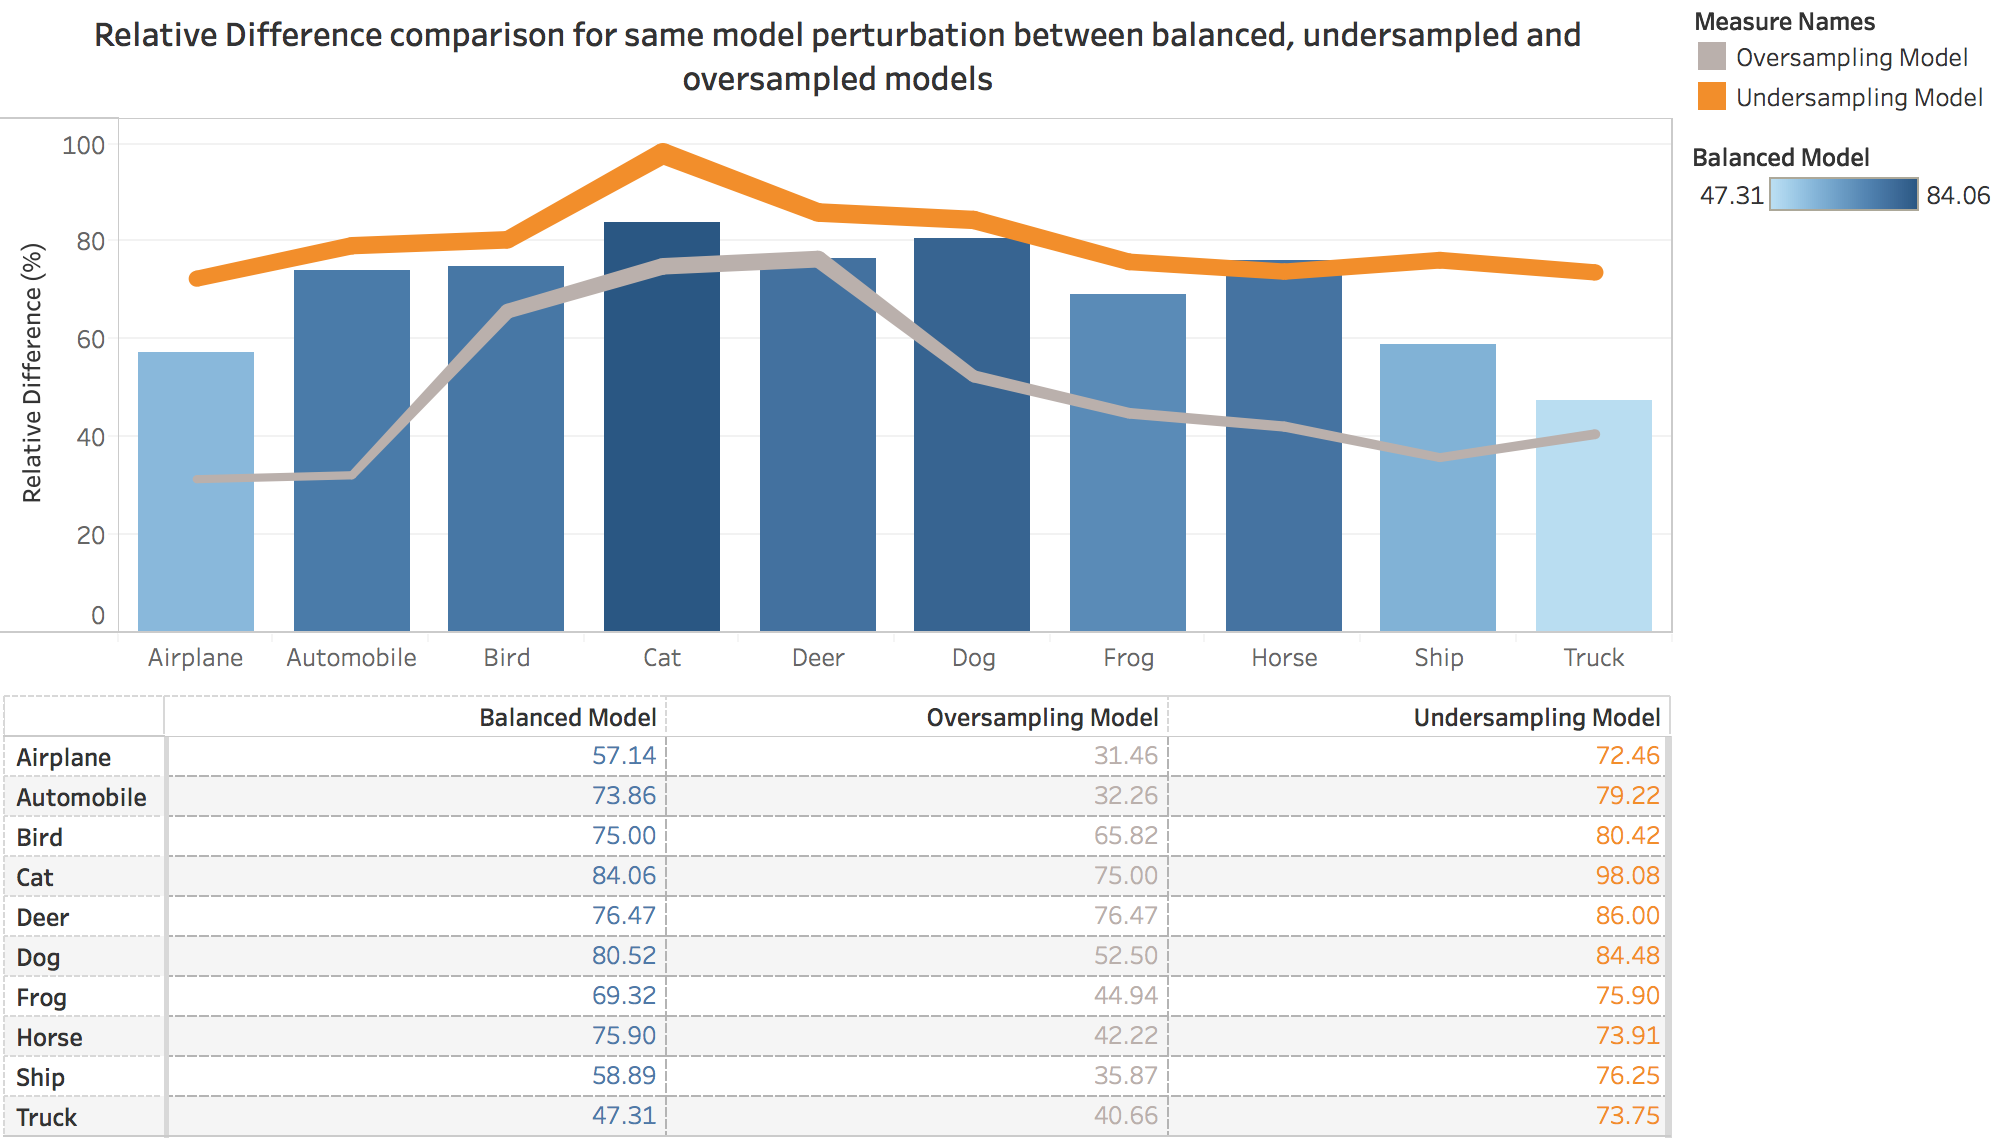
\includegraphics[scale=0.3]{rel_diff_graph.png}
	\caption{Relative difference for each model. Higher numbers means more vulnerability}
	\label{fig:relative_difference}
\end{figure}
Chapter 4 discussed different ways in which a new model could learn from existing ones. Black-box attack is when the attacker has no knowledge of the underlying model that he/she wants to attack and the best way to learn the gradient information is by querying the target and training a new model with its outputs. White-box attack is when the same model is used to extract the gradient for the gradient sign method. Our Black-box experiments has a slightly different configuration, as we use a modified version of the dataset to train a different model.


The use of a different model (black-box) for creating adversaries has shown less effective when compared to the same model (white-box) attack. As the overall gradient have not only different direction but also magnitudes, the attacked system has proven to be more robust. The experiment reveals that although gradient sign method is quite effective for fooling networks it does require a good amount of knowledge from the underlying training parameters so as to unleash its full potential.
\begin{figure}
	\centering
	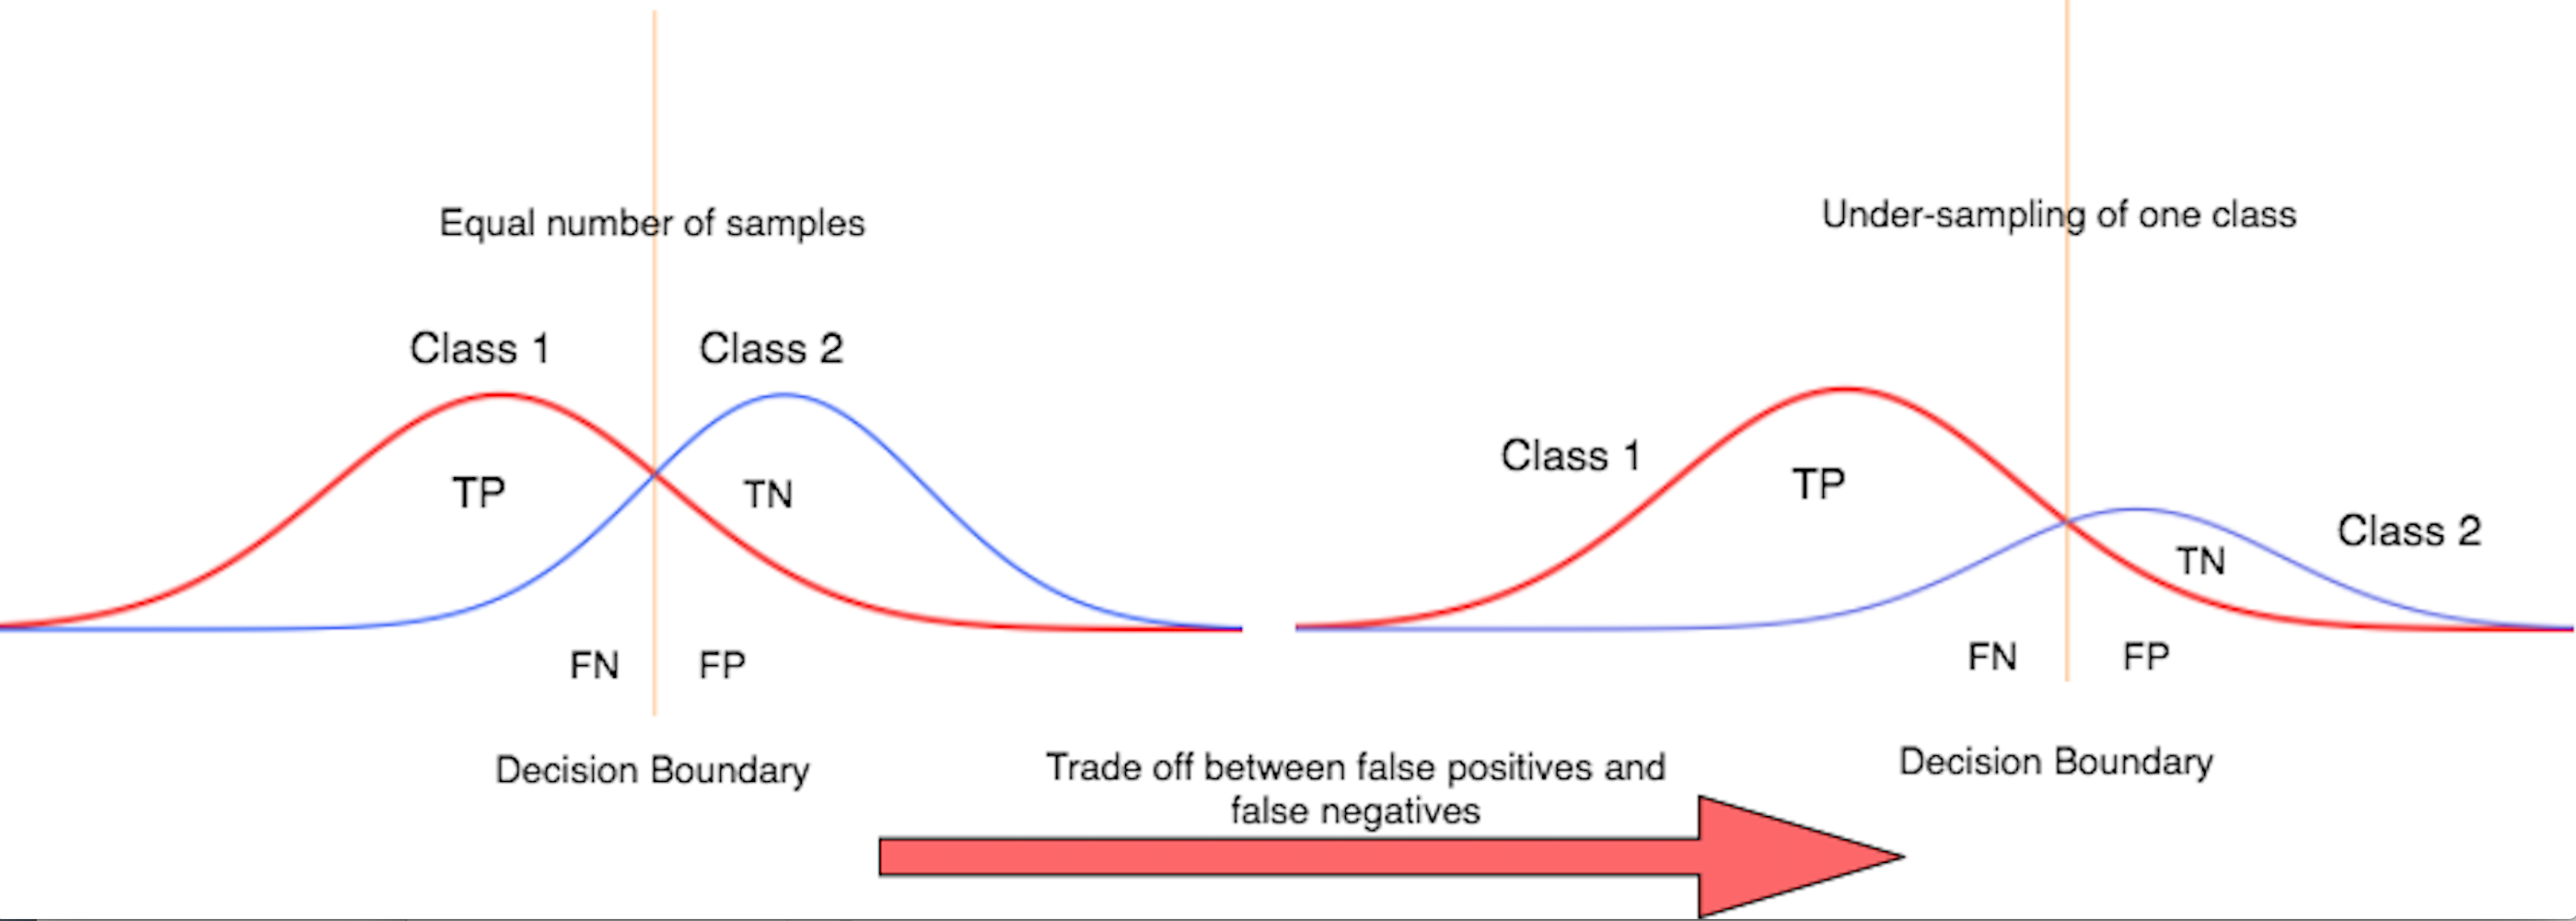
\includegraphics[scale=0.32]{class_dist.png}
	\caption{Dataset imbalance causes models to perform adjustments of decision boundaries leading to an increase on accuracy of the majority class and decrease on the minority class.}
	\label{fig:class_dist}
\end{figure}
Attacking an under-sampled target with the gradient of a balanced model did not show to be as effective as using the same model's gradient. The average accuracy of the under-sampled attack with adversaries generated from a different network was 53.8\% while the same metric was 25.8\% for the white-box attack. Even that our training samples are within the same data domain, there are still huge differences on the gradients learned from each model. 

Due to the high dimensionality of CNN models, every training process learns different weights and biases that could equally generalise for all classes. As these are not guaranteed to converge to global optima, several different local optima could be found by the same optimisation procedure. Therefore, black-box adversary generation is not using the true target gradient directions, as they were submitted, in our case, to different optimisation stage and different dataset configuration.

Our experiments shows that gradient information is extremely important to gradient sign methods. Both the over-sampling of specific classes on the datasets and the model internal knowledge increases robustness to gradient sign methods. This shows that high quality datasets with equal number of samples per class are one way of avoiding the degradation of real-life systems performance when attacked by adversarial methods.

\section{Overlapping distributions}
The results for the balanced network on figure~\ref{fig:conf_matrix_full} shows that for the pairs cat/dog and automobile/truck there is already a natural misclassification between one another. For instance 13\% of dog samples were misclassified as cat in the original balanced model. Our experiment demonstrates that the adversarial attacks intensify this phenomena in only one of the classes of the pair. While for both under-sampled cat and truck the number of samples misclassified with the similar class has increased, the same did not happen with dog and automobile. Figure~\ref{fig:overlap} shows that cats are increasingly misclassified as dogs when under-sampling on the cat class is used. While on the cat under-sampling case the percentage of samples misclassified as dogs increased from 31\% to 39\%, the same number decreased from 38\% to 32\% on the dog under-sampling test.

\begin{figure}
	\centering
	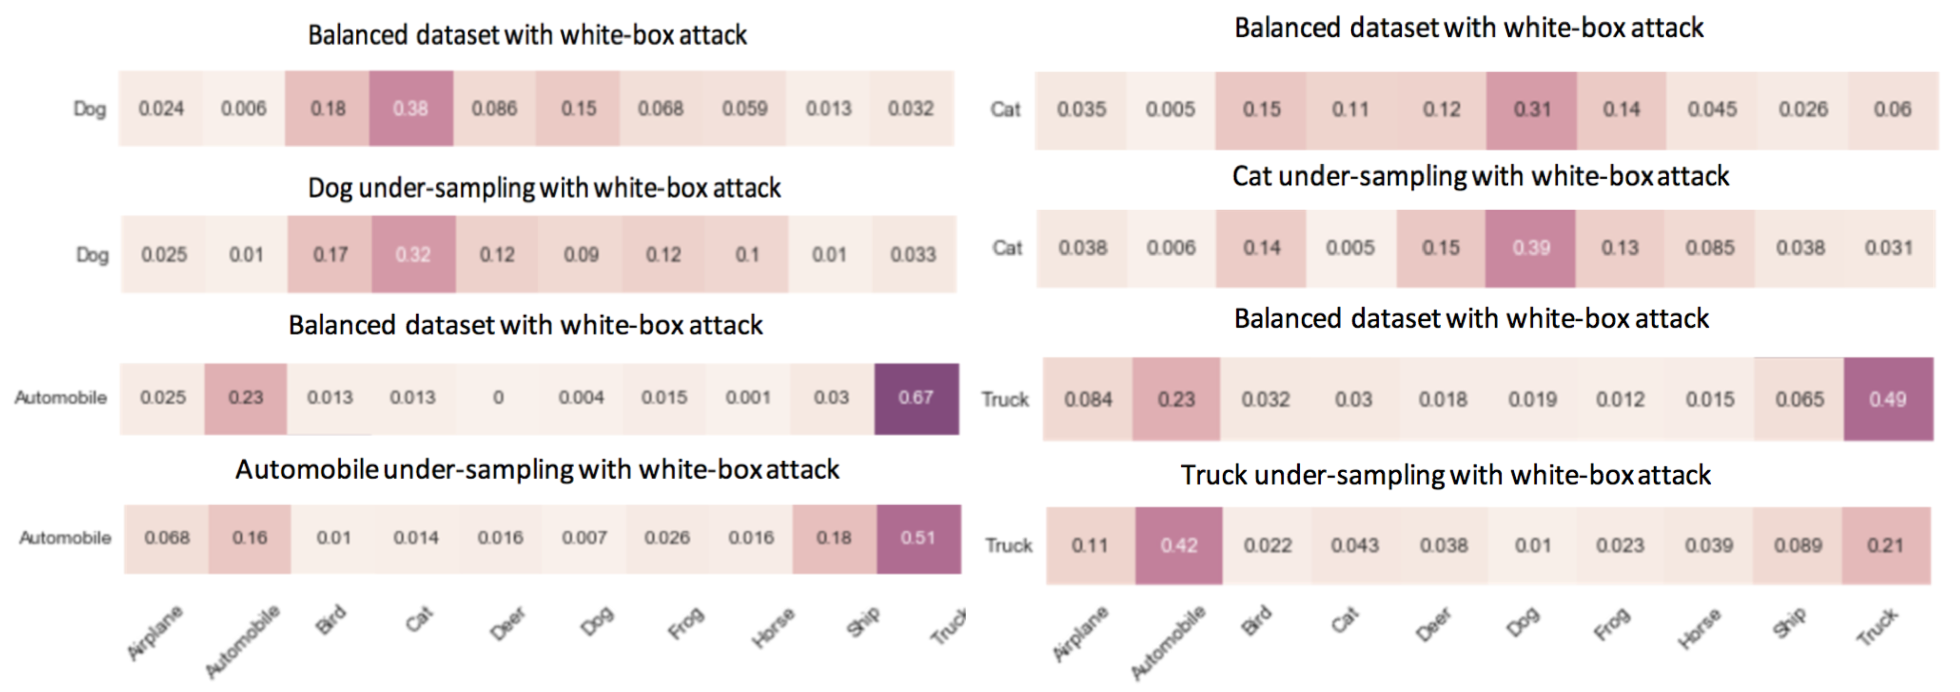
\includegraphics[height=5.5cm]{overlapping_all.png}
	\caption{Under-sample on cat and truck increases misclassification to similar classes, while dog and automobile does not.}
	\label{fig:overlap}
\end{figure}

The most important features of the affected pair seems to overlap so as to this phenomena to happen. It is hard to reason with distributions on high-dimensional spaces, however, the results shows that linear behavior is achieved even on non-linear environments. This confirms previous works discoveries that although CNNs are made of non-linearities, they still perform linearly in most cases. Classes with overlapping distributions shows that decision boundaries of high-dimensional models are as fragile as the ones learned on linear models. One way to explain this is by looking at the activation functions of current CNNs architectures. They are usually made of RELU or TANH, which is a step function with somewhat linear behavior. The stacking of such functions create a high-dimensional linear space, where methods like the gradient sign are able to perform well by intentionally causing domain shift on data points that are close together in space.

\chapter{Conclusion and future work} \label{chap:conclusion}
In this work we have presented how adversarial attacks using the gradient sign method with ascent perturbations perform on CNNs trained on imbalanced datasets using the same and different model gradients. Neural networks and convolutional neural networks were explained in details in chapter 1 followed on the next chapter by the adversarial attacks taxonomy and imbalanced learning problem implications to machine learning methods. Types of adversarial attacks were then presented, showing that black-box attacks are successful on real-world systems and the implications of model internal knowledge to the gradient sign method. Chapters 5 an d 6 were dedicated to showing the details of our experiment design and to present and discuss the results on all of our models.

Adversarial methods were proven to increase the domain shift effect on test datasets as it is explained by \cite{papernot2016transf}. We have shown that adversarial attacks are even more severe on datasets with under-sampled class labels and that the decision boundary trade-off on the over-sampled classes increases their robustness to adversarial examples. Labels with similar features have only shown higher vulnerability to the fast gradient sign methods in one of the classes of the pair. This specific result shows that similar classes might have degrees of similarities on which could be more or less exploited by the gradient method.  

Convolutional neural networks have been adopted more widely as the current techniques improve. However, understanding of such methods is hard as the number of degrees of freedom in the model hinders thorough analysis. Until now, most people  are used to see these models as black-boxes, since they can not reason about the causality relationship between the model performance and its internal knowledge. The highly non-linear structure and state of the art performance of CNNs do not shield them from one of the most common effects in machine learning models - the domain shift caused by unseen data points.

As several commercial applications rely on almost the same group of models, understanding of such properties is of extreme importance. Future work in this field could look further in datasets with a higher number of classes and more complex relationships between labels so as to not only confirm our insights but also discover new interesting properties of class imbalanced CNNs and adversarial attacks. Current applications looking to increase their robustness to adversarial attacks could use over-sampling techniques on critical labels so as to shield that label from malicious attacks.

This work sheds an important light on machine learning methods. Several real-life models are deeply concerned with possible vulnerabilities of their system, and studies on this field were being done for the past years. Still, the imbalance learning problem remains one of the big questions in machine learning. Current applications looking to increase their robustness to adversarial attacks could use over-sampling techniques on critical labels so as to shield that label from malicious attacks




%%%%%%%%%%%%
% End

% Bibliography
\bibliographystyle{style/mybibstyle}
{
\setstretch{1.25}
\cleardoublepage
\phantomsection
\bibliography{refs}
}

%%%% Appendices
%%%\appendix
%%%\addtocontents{toc}{\protect\setcounter{tocdepth}{1}}
%%%\input{wikifeats/wikifeats.tex}
%%%\input{candcner/candcner.tex}
%%%\input{comparedata/comparedata.tex}

\end{document}
